\documentclass[final]{ukthesis}
%you must include these 2 packages.
\usepackage[pdfauthor={Sen Li},
            pdftitle={Universal Real-Time XYZ rectified Reconstruction for RGB-D Cameras},
            pdfsubject={3D Camera Calibration},
            pdfkeywords={3D Reconstruction; Camera Calibration; RGBD; Image Processing},
            pdfproducer={Latex with hyperref},
            pdfcreator={latex->dvips->ps2pdf},
            pdfpagemode=UseOutlines,
            bookmarksopen=true,
            letterpaper,
		hidelinks,
            bookmarksnumbered=true]{hyperref}
\usepackage{memhfixc}

\usepackage{mathptmx}% http://ctan.org/pkg/mathptmx
\usepackage{amsmath}
\usepackage{graphicx}
\usepackage[lofdepth,lotdepth]{subfig}
\usepackage{textcomp}
\usepackage{amssymb}
\usepackage{caption}
\usepackage{float}

\DisemulatePackage{setspace}
\usepackage{setspace}

\usepackage[autostyle=true]{csquotes} % Required to generate language-dependent quotes in the bibliography
\graphicspath{{Figures/}{./}} % Specifies where to look for included images

\usepackage{multirow}
\usepackage{makecell}
\usepackage{varwidth}
\setcounter{MaxMatrixCols}{20}

%\usepackage{amsxtra}     % Use various AMS packages
%\usepackage{amssymb}
%\usepackage{amsfonts}
%\usepackage{graphicx}    % Add some packages for figures. Read epslatex.pdf on ctan.tug.org
%\usepackage{rotating}
%\usepackage{color}
%\usepackage{epsfig}
%\usepackage{verbatim}
%\usepackage{natbib}      % Allows you to use BibTeX
%\usepackage[printonlyused]{acronym} 

%%%%%%%%%%%%%%%%%%%%%%%%%%%%%%%%%%%%%%%%%%%%%%%%
\begin{document}
%author data  Electrical Engineering
\author{Sen Li}
\title{Universal Real-Time XYZ Calibrated Reconstruction\\ for RGB-D Cameras}
\abstract{%
Ever since the Kinect brought low-cost depth cameras into consumer market, with PrimeSense 3D
sensing technology as the core depth determination principle for its first generation,
great interest has been invigorated into RGB-D sensors. However, there has not been a systematic solution to combine both of 3D reconstruction and the radial dominated lens distortions correction. What is worse, the traditional pinhole-camera-model based 3D camera calibration method does not consider the depth distortion. In this thesis, a data-based look-up table software calibration method is proposed to do real-time rectified 3D reconstruction for universal RGB-D cameras. The idea is inspired and extended from a structured light real-time 3D reconstruction system. A transition from pinhole-camera calibration model to data-based lens distortion-removed calibration model is analyzed. High-order polynomial surface mapping is employed for non-linear distortion correction, and an individual Bluetooth Low Energy Optical-Flow tracking module is introduced for external \(Z^w\) value support.
}
\advisor{Dr. Daniel L. Lau}
\keywords{3D Reconstruction; Camera Calibration; RGBD; Image Processing}
\dgs{Dr. Caicheng Lu}


%the title pages
\frontmatter
%\maketitle


%\begin{acknowledgments}
%Acknowledge people/things here
%\end{acknowledgments}
%\begin{dedication}
%Dedicated to things (optional)
%\end{dedication}


\tableofcontents\clearpage
\listoffigures\clearpage
\listoftables\clearpage


%----------------------------------------------
\mainmatter

\onehalfspacing

%% Chapter 1
\chapter{Introduction} % Main chapter title
\label{sens_introduction} % For referencing the chapter elsewhere, use \ref{sens_introduction} 
%%%%%%%%%%%%%%%%%%%%%%%%%%%%%%%%%%%%%%%%%%%%%%%%%
%%%%%%%%%%                                                     %%%%%%%%%%%%%%%%%%%%%%%%%%%
%%%%%%%%%%           1.1   Depth Camera Application                   %%%%%%%%%%%%%%%%%%%%
%%%%%%%%%%                                                     %%%%%%%%%%%%%%%%%%%%%%%%
%%%%%%%%%%%%%%%%%%%%%%%%%%%%%%%%%%%%%%%%%%%%%%%%%%
\section{Depth Camera Application}

As the depth camera technology opens a new epoch for three-dimensional (3D) markets, the multimedia technologies development is changing from two-dimensional (2D) to 3D on games, movies, health care aid, military training, etc., all various areas that are in demand of a more direct reflection on the real world \cite{depthOverview12}. Simple 2D scenes are not able to meet the social demands any more. And with the fast development of multimedia technologies, three-dimensional (3D) scene display has become a hotspot in the display field. As an extension of classic 2D video, the 3D dynamic display technology can provide a more comprehensive immersive feeling to users than a 2D video. Gesture recognition, 3D modeling, 3D printing, augmented reality, virtual reality, etc., a lot of ongoing researches and applications on depth cameras are famous now, cooperated with Human Computer Interaction (HCI) technologies.
\\\\%
Pattern recognition and gesture recognition are of the hottest sustained research activities in the area of HCI. Being a significant part in non verbal communication hand gestures are playing vital role in our daily life. Hand Gesture recognition system provides us an innovative, natural, user friendly way of interaction with the computer which is more familiar to the human beings. Gesture Recognition has a wide area of application including human machine interaction, sign language, immersive game technology etc. By keeping in mind the similarities of human hand shape with four fingers and one thumb, \cite{gestureRecognition12} present a real time system for hand gesture recognition on the basis of detection of some meaningful shape based features like orientation, center of mass (centroid), status of fingers, thumb in terms of raised or folded fingers of hand and their respective location in image.
\\%
Since gestures based on hand and finger movements can be robustly understood by computers by using a special 3D IR camera, users are allowed to play games and interact with computer applications in natural and immersive ways that improve the user experience. In 2010, Microsoft's first generation Kinect, using PrimeSense’s technology, is based on projecting a structured light pattern on the object in order to build and track the skeleton of the user’s body to control a series of electronic games. \cite{SL3Dfrom2D96} also discussed similar techniques for 3D object reconstruction. By using this depth-map along with the 2D color images obtained via the Kinect camera, the computational unit of the Xbox 360 console was capable of providing a fairly robust gesture recognition solution. After \cite{KinectGesture12} proposed two methods for gesture recognition, a plethora of applications have been produced around Kinect by various groups of image processing researchers.
\\%
A Kinect-based calling gesture recognition scenario is proposed by \cite{gestureKinect14} for taking order service of an elderly care robot. Its proposed scenarios are designed mainly for helping non expert users like elderly to call service robot for their service request. In order to facilitate elderly service, natural calling gestures are designed to interact with the robot. Individual people is segmented out from 3D point cloud acquired by Microsoft Kinect, skeleton is generated for each segment, face detection is applied to identify whether the segment is human or not, specific natural calling gestures are designed based on skeleton joints. \cite{NIRGesture14} proposed another smart and real-time depth camera based on a new depth generation principle. A monotonic increasing and decreasing function is used to control the frequency and duty-cycle of the NIR illumination pulses. The adjusted light pulses reflect off of the object of interest and are captured as a series of images. A reconfigurable hardware architecture calculates the depth-map of the visible face of the object in real-time from a number of images. The final depth map is then used for gesture detection, tracking and recognition.
\\\\%
3D printing is an additive technology in which 3D objects are created using layering techniques of different materials, such as plastic, metal, etc.  It has been around for decades, but only recently is available and famous among the general public. The first 3D printing technology developed in the 1980’s was stereolithography (SLA) \cite{Patent3Dprinting86}. This technique uses an ultraviolet (UV) curable polymer resin and an UV laser to build each layer one by one. Since then other 3D printing technologies have been introduced.
%
Nowadays, some companies like iMaterialise or Shapeways offer 3D printing services where you can simply upload your CAD model on-line, choose a material and in a few weeks your 3D printed object will be delivered to your address. This procedure is quite straight-forward when you got your CAD model. However, 3D shape design tends to be a long and tedious process, with the design of a detailed 3D part usually requiring multiple revisions. Fabricating physical prototypes using low cost 3D fabrication technologies at intermediate stages of the design process is now a common practice, which helps the designer discover errors, and to incrementally refine the design. Most often, implementing the required changes directly in the computer model, within the 3D modeling software, is more difficult and time consuming than modifying the physical model directly using hand cutting, caving and sculpting tools, power tools, or machine tools. When one of the two models is modified, the changes need to be transferred to the other model, a process we refer to as synchronization. Changes made to the computer model can be transferred to the physical model by 3d printing a new physical model. \cite{3DPrintingFrom3DSensing13} proposed and introduced a from-Sense-to-Print system that can automatically generate ready-to-print 3D CAD models of objects or humans from 3D reconstructions using the low-cost Kinect sensor. Further, \cite{3DModelingForPrinting15} addresses the problem of synchronizing the computer model to changes made in the physical model by 3D scanning the modified physical model, automatically detecting the changes, and updating the computer model. A new method is proposed that allows the designer to move fluidly from the physical model (for example his 3D printed object, or his carved object) to the computer model. In the proposed process the physical modification applied by the designer to the physical model are detected by 3D scanning the physical model and comparing the scan to the computer model. Then the changes are reflected in the computer model. The designer can apply further changes either to the computer model or to the physical model. Changes made to the computer model can be synchronized to the physical model by 3D printing a new physical model.

%%%%%%%%%%%%%%%%%%%%%%%%%%%%%%%%%%%%%%%%%%%%%%%%%
%%%%%%%%%%                                                                %%%%%%%%%%%%%%%%%
%%%%%%%%%     1.2  3D Reconstruction of RGB-D Cameras    %%%%%%%%%%%%%%%%%%%%
%%%%%%%%%%                                                                %%%%%%%%%%%%%%%%%%
%%%%%%%%%%%%%%%%%%%%%%%%%%%%%%%%%%%%%%%%%%%%%%%%%%
\section{3D Reconstruction of RGB-D Cameras}

3D reconstruction aims to reproduce the 3D profile of real objects as accurate as possible, which require accurate world coordinate \(X\)/\(Y\)/\(Z\) (noted as \(X^{w}\)/\(Y^{w}\)/\(Z^{w}\)  henceforth) values in three dimensional space for every single point of a profile. Ever since the Kinect brought low-cost depth cameras into consumer market, with PrimeSense 3D sensing technology as the core depth determination principle for its first generation, great interest has been invigorated into RGB-D sensors. Camera calibration is a necessary part in 3D reconstruction in order to extract metric information from 3D images, i.e., to determine a translation from \(Z^{w}\) to \(X^{w}\)/\(Y^{w}\)  for every pixel based on its row and column. In the mean time, optical and perspective distortion become a problem that stops from getting a good view. On most wide angle prime lenses and many zoom lenses with relatively short focal lengths,  especially cheap low quality lenses, barrel distortion would typically be present. In this research, a more accurate novel method with precise calibration system is brought in for real-time rectification and 3D reconstruction of universal RGB-D cameras. 

\begin{table}[ht]
\begin{center}
\caption{ 3D profile acquisition Taxonomy}
\label{3DImagingTaxonomy}
\hspace*{-1cm}
\begin{tabular}{ |>{\small}l|>{\small}l|>{\small}l|>{\small}l| }
\hline
\multicolumn{4}{|c|}{3D Shape Extraction} \\
\hline
\multicolumn{2}{|c|}{Passive}  & \multicolumn{2}{c|}{Active}\\
\hline
Single Vantage Point & Multiple Vantage Points & Single Vantage Point & Multiple Vantage Points\\
\hline
\multirow{5}{*}{
\makecell[l]{
\textbullet \, Shape from Texture\\ 
\textbullet \, Shape from Occlusion\\
\textbullet \, Time to Contact\\
\textbullet \, Shape from Defocus\\
\textbullet \, Shape from Contour}
} 
&
\multirow{5}{*}{\makecell[l]{
\textbullet \, Passive Stereo\\ 
\textbullet \, Structure from Motion\\
\textbullet \, Shape from Silhouettes}
}
&
\multirow{5}{*}{\makecell[l]{
\textbullet \, Time of Flight\\ 
\textbullet \, Shape from Shading}
} 
&
\multirow{5}{*}{\makecell[l]{
\textbullet \, Structured Light\\ 
\textbullet \, Active Stereo\\
\textbullet \, Photometric Stereo}
} \\ & & &
\\ & & &	\\ & & &	\\ & & &\\
\hline

\end{tabular}
\end{center}
\end{table}

%
\noindent
Three dimensional (3D) profile measurement technologies have been developed by various means, as summarized by Theo Moons \cite{CourseNotes}, among which the non-contact optical methods are widely applied into reality as consumer RGB-D camera. Traditionally, with Pinhole camera model, as the basics of camera calibration, to supply the translation from \(Z^{w}\)  to \(X^{w}\)/\(Y^{w}\) , the core procedure of 3D Reconstruction falls on the determination of per-pixel depth to serve as \(Z^{w}\) .%
%\par%
%\noindent
Within the non-contact optical category, as well as 3D reconstruction using multiple images, there are two levels of distinctions, as shown in the 3D profile acquisition taxonomy diagram \cite{Reconstruction10} given in table \ref{3DImagingTaxonomy}. 
\\\\%
The first distinction: active methods and passive methods. Their classifications are decided by the control of light sources. Active methods need special light sources control as part of the strategy to get 3D information, while on the other hand, passive techniques could work with whichever reasonable available ambient light. With a special known illumination offering more information to simplify some of the steps for 3D information acquiring process, active methods tend to be computationally less demanding. Both of the famous consumer PrimeSense and KinectV2 3D cameras, which are calibrated by the new proposed approach, are using active methods.
 %\\\\
The second distinction: single-vantage points methods and multi-vantage points methods. The second distinction is determined by the number of vantage points. With a single vantage system, reconstruction is done based on single view point. In the case that there are multiple viewing or illumination components, all of them would be positioned very close to each other so that they could ideally coincide. For multi-vantage points methods, several viewpoints, with possible controlled illumination source positions, are involved. As contrast with the single-vantage points methods, the multi-vantage systems need the different components to be positioned far enough from each other. 
%\\\\
Among the above non-contact optical methods, structured-light and time-of-flight methods are of the most practical importance.
As will be discussed shortly, the PrimeSense technology and SeikowaveLCG camera use Stuctured light methods, and the KniectV2 camera uses Time-of Flight. 
\\
\\\textbf{Structured Light}\\
Structured light (SL) based techniques are famous for its fast speed. It is composed of one camera and one light pattern projector \cite{Kai10}. The projector projects a series of special known patterns onto a target, and the camera captures the corresponding images, which contain special information corresponded to the patterns from the projector. A decoding algorithm would be used to extract world coordinate information of the target object from the captured images, by analyzing the relationship among the camera, the projector and the target object using triangulation.\\
\\
Being after accuracy, the most important issue for structured light method comes to the question of, how to design the projected patterns. In other words, how to design the coding algorithm and its corresponding decoding strategy will decide the final quality of the reconstructed 3D profile. Various classified SL pattern strategies have been proposed, and are still being studied.
\\
Figure \ref{PrimeSenseInfraredPattern} shows the an infrared speckle pattern that is projected onto a target by the infrared projector of PrimeSense 3D scanner,\par
%
\begin{figure}[H]
\centering
\includegraphics[width=0.8\textwidth]{PrimeSenseInfraredPattern}
\caption[PrimeSense SL Infrared Pattern.]{
\begin{varwidth}[t]{\linewidth}
PrimeSense SL Infrared Pattern. \\%
Source: \url{http://www.ros.org/wiki/kinect_calibration/technical}
\end{varwidth}
}
\label{PrimeSenseInfraredPattern}
\end{figure}%
%
and an infrared camera inside the scanner is employed to capture images of the target. By comparing part by part to reference patterns, that were captured previously at known depths and stored in the device, the per-pixel depth could be looked up based on the reference pattern that the projected pattern matches best. 
%\\\\
After the per-pixel depth data determined from the infrared sensor, the next step would be to correlate to a calibrated RGB data, which will generate a popular unified representation of target's profile: point cloud, a collection of points with \(XYZ\) 3D coordinates and RGB color data. What's more, the surface normals of the target's profile are also stored in every single point of the point cloud data. 
%
\\
\\\textbf{Time of Flight (KinectV2)}\\
Based on known speed of light, Time-of-Flight (ToF) camera resolves distance by measuring the time cost of a special light signal traveling between the camera and target for every single point. KinectV2 is one of the practical consumer 3D camera that applied the technology of ToF. Using the active modulated infrared source light together with a low-cost CMOS pixel array, KinectV2 realize its an attractive solution that owns compact construction, high accuracy and up to 30 fps frame-rate.\par%
%
%
\begin{figure}[H]
\centering
\includegraphics[width=0.7\textwidth]{timeOfFlight}
\caption{3D time-of-flight camera operation \cite{TimeOfFlight}}
\label{timeOfFlight}
\end{figure}%
%
\noindent
The variable that ToF camera measures is the phase shift between the illumination and reflection, which will be translated to distance \cite{TimeOfFlight}. % Texas Instruments Time-of-Flight Camera -An Introduction    Larray Li
To detect the phase shifts, light source is pulsed or modulated by a continuous wave, typically a sinusoid or square wave.
As figure \ref{timeOfFlight} shows, the ToF camera illumination is typically from a LED or a solid-state laser operating in the near-infrared range invisible to human eyes. A camera working in the same spectrum captures the reflected light and converts photonic energy to electrical signal, which contains distance (depth) information.
%\\\\
The distance measured for every single pixel is saved into a 2D addressable array, which results in a depth map. KinectV2 has a depth map of 512 * 424 unsigned short data collections, which could be finally rendered, together with corresponded RGB stream,  into a tree dimensional space point cloud.
%%%%%%%%%%%%%%%%%%%%%%%%%%%%%%%%%%%%%%%%%%%%%%%%%%%%%%
%%%%%%%%%%                                                                         %%%%%%%%%%%%%%%%%%%%
%%%%%%%%%%  1.3   Structured Light 3D Scanner Calibration       %%%%%%%%%%%%%%%%%%%%
%%%%%%%%%%                                                                            %%%%%%%%%%%%%
%%%%%%%%%%%%%%%%%%%%%%%%%%%%%%%%%%%%%%%%%%%%%%%%%%%%%%%

\section{Structured Light 3D Scanner} % (specially with cheap low quality lenses)
\label{sectionSL3DCalibration} % For referencing the chapter elsewhere, use \ref{sectionSL3DCalibration} 

Structured Light Illumination (SLI) has become the most widely used active vision [12] method for non-contact 3D measurement, applied in the fields of industrial quality control [14, 15], biometrics [16], biomedical topology [13],  archaeologicaldocumentation [9],  and the entertainment industry.  The numerous uses of SLI have lead to an abundance of different methods for the generation of surface topology, although each technique utilizes the basic premise of measuring the specific deformation of a projected light pattern on the surface contours of a target object [17].  The light pattern can take various forms: a spot [12], a single light stripe [17, 18], multiple light stripes[19], a grid[20,21], sine-wave encoded stripes[22], binary encoded stripes, and various other patterns [12].

The way a pattern is utilized to generate 3D information can vary as well, evolving from the classic SLI approach utilizing a single light stripe.  In this classic approach, a single laser stripe is scanned laterally across a surface and a 2D image is captured for each of the points that the stripe intersects.  This causes the 3-D resolution to be directly related to the number if images captured, and drives the inherent costs of processing the data very high.  Improved methods utilizing multiple stripes [19] can capitalize on illuminating the entire surfacein the captured image to gain increased performance,butthese multi-striped patterns introduce ambiguities near discontinuities in the target surface, and can be sensitive to the albedo of the surface.  Using multi-frame pattern techniques in a sequence, each pixel of the image can be encoded to eliminate the reconstruction ambiguities and sensitivity to the albedo surface.  The sequences can consist of color-encoding patterns [23] or binary-encoding patterns [27, 28], but the multi-frame pattern sequence called phase-measuring Profilometry (PMP) [29]is particularly robust and the focus of this Thesis.

PMP encodes the surface points with specific phase values, with increasing depth resolution when using higher frequency patterns.  The downside is that ambiguous reconstruction occurs with higher frequencies, which leads to multiple-frequency PMP techniques [30-32] to resolve the ambiguities with the phase.Using a conventional PMP method, erroneous motion of the target surface causes reconstruction artifacts that are unresolvable; however, a method called Lock and Hold [40, 41]allows thecapture of full 3-D motion with the depth-resolution of a high frequency PMP pattern.   








Structured light (SL) technique is the fastest method for 3D reconstruction. By driving the projector / camera pair at very high frame rates, the object's motion then become small over the pattern set. However, at a high frame rate, the process speed of incoming video becomes an issue. Instead of recoding camera frames to memory and then applying off-line processing (like many video-based SL systems chose), Kai \cite{Kai10} made a good research on structured light 3D reconstruction in real-time, which brought in a pinhole-camera model based 3D scanner calibration method. %
%\\\\%
To be able to produce 3D point clouds in real-time, Kai proposed a look-up table based solution that is built on the derivation of pinhole camera model 3-by-4 transformation matrix, with a novel dual-frequency pattern. By his method, a 640 by 480 video steam can generate intermediate phase data at 1063.8 frames per second and full 3D coordinate point clouds at 228.3 frames per second, which is a satisfying speed. However, this method, being not able to remove lens distortions, is only one good lead-in 3D camera calibration method.%
\\\\%
3D scanner calibration aims to determine the mathematical equation for every single pixel's sight, i.e., to calculate a beam equation. Concretely, with \enquote{depth} (\(Z^{w}\)) value given in RGB-D cameras, the beam equation calculation is to determine the linear translation coefficients from \(Z^{w}\) to \(X^{w}\) and \(Y^{w}\). And how well the calibration is depends on how much distortions are removed in the beam equation.%
%\\\\%
Two kinds of distortions need to be taken care of through 3D camera calibration: perspective distortion and lens distortion. Perspective distortion is caused by the position of the camera relative to the subject, or by the position of the subject within the image frame, linear. And lens distortion is caused by optical design of lenses, non-linear. Traditionally and commonly, an ideal pinhole camera model is employed as an simple algorithm in 3D computer vision to describe a mapping from the 3D world coordinates to camera image row and column, by giving a translation method from \(Z^{w}\) to \(X^{w}\)  and \(Y^{w}\)  for every single pixel. It works decently only for ideal pinhole cameras that have no lens, whereas real cameras need extra modifications and supplementations to solve the non-linear radial and tangential lens distortion.%
%\\\\%
Totally based on the pinhole camera model (a 3-by-4 matrix), the 3D camera calibration method from Kai's analysis can only take care of the linear perspective distortion, which not able to handle the non-linear radial dominated lens distortion. Details will soon be discussed in in chapter \ref{sens_PinHoleCameraStructuredLight}. %
%
%
%
%%%%%%%%%%%%%%%%%%%%%%%%%%%%%%%%%%%%%%%%%%%%%%%%%%%%%%%
%%%%%%%%%%                                                     %%%%%%%%%%%%%%%%%%%%%%%%%%%
%%%%%%%%%%  1.3   Contributions of this thesis             %%%%%%%%%%%%%%%%%%%%%%%%
%%%%%%%%%%                                                     %%%%%%%%%%%%%%%%%%%%%%%%
%%%%%%%%%%%%%%%%%%%%%%%%%%%%%%%%%%%%%%%%%%%%%%%%%%%%%%%
\section{Contributions of this thesis}
%%%%%%	
For RGB-D cameras, RGB steam and Depth steam are two steams that independent but correlated with each other. With respect to every \(X^{w}\)/\(Y^{w}\) correlated single pixel-pair, Depth steam offers the additional voxel world coordinates \(Z^{w}\), while RGB steam offers the additive color property.
%\\\\
As described in section \ref{sectionSL3DCalibration}, even though a pinhole camera model (3-by-4 transformation matrix) could help do 3D scanner calibration, it is only for ideal camera without lens. That is to say, in practical the lens distortions correction is separated from pinhole camera model calibration. Even though same pixel coordinate-pairs (world coordinates and image plane coordinates) could be re-utilized to solve radial dominated lens distortions, as a second step after the determination of a 3-by-4 pinhole camera model, the calculation of the separated step brings a second-time translation cost for every single pixel of every frame. This is not a good way to do real-time reconstruction. %
\\\\%
In order to remove the radial dominated lens distortions, two 3D camera calibration methods, got inspired from Kai's method, are proposed and discussed. The first method inherits the advantages given by the pinhole camera model, which can offer the relationship between \(Z^{w}\) and \(X^{w}\)/\(Y^{w}\) for every single pixel as long as its field of view is pre-calculated. This method is only discussed theoretically, because the second method is simpler, more accurate, and is finally applied into practical calibration.%
%\\\\%
Thoroughly abandoned the pinhole camera model, the second method directly determines the beam equation for every single pixel by collecting distortions-removed \(X^{w}\)/\(Y^{w}\) and accurate \(Z^{w}\) values. \(X^{w}\)/\(Y^{w}\) values are calibrated by high order, concretely \(4th\) order, polynomial surface mapping. And the accurate \(Z^{w}\) values are imported from external \(Z^{w}\)-aixs tracking module. In short, this is totally a data-based calibration method.%
%
\begin{figure}[H]
\centering
\includegraphics[width=0.5\textwidth]{trackingModuleOnKinectV2CalibrationSystem}
\caption{KinectV2 Calibration System}
\label{trackingModuleOnKinectV2CalibrationSystem}
\end{figure}%
%
\noindent
To collect enough data along \(Z^{w}\)-aixs, a rail is used in the calibration system. As shown in figure \ref{trackingModuleOnKinectV2CalibrationSystem}, the rail is perpendicular to the uniform round dot pattern as \(Z^{w}\) axis. A RGB-D camera KinectV2 is mounted on the top of the slider, while a BLE OF tracking module is specially designed and mounted at the bottom of the slider, observing the rail and supporting accurate \(Z^{w}\) values. With this calibration system that helps collect data easily, a distortion-removed XYZ-D Look-Up Table (LUT) will be generated for real-time 3D reconstruction.%
%%%%%%%%%%%%%%%%%
%%%%%%%%%%%%%%%%%
%%%%%%%%%%%%%%%%%
%%%%%%%%%%%%%%%%%

\section{Summation}

 RGB-D cameras' calibration cannot be easily handled by a pinhole camera model. First of all, as mentioned in section \ref{sectionSL3DCalibration} and detailed in section \ref{sectionPinholeCamera}, a pinhole camera model is not able to handle the non-linear radial dominated lens distortion. What's worse, the depth resolution deteriorates notably with depth in practical \cite{Krystof12}, so such so that the \(depth\) values are not able to guarantee an accurate  \(Z^{w}\).
%
 \begin{figure}[H]
%\centering
\subfloat[Front View][Front View]{
\includegraphics[height=0.42\textwidth]{NIR_by_Depth_front}
\label{NIR_by_Depth_front}}
\subfloat[Left View][Left View]{
\includegraphics[height=0.42\textwidth , width = 0.4\textwidth]{NIR_by_Depth_LeftSide}
\label{NIR_by_Depth_LeftSide}}
%\qquad
\caption{Raw NearIR 3D Reconstruction based on Pinhole Camera Model}
\label{NearIR}
\end{figure}%
%
\noindent
Noises among depth data vary randomly, camera by camera and pixel by pixel; which means a rough point-cloud plane full of bumps and hollows will be reconstructed even though the camera is observing a wall. As shown in figure \ref{NIR_by_Depth_LeftSide}, the blue straight line should be the left side of the 3D reconstruction, whereas most pixels on the left side border are apparently not sitting on a straight line.%
%
Got inspired and extended from Kai's 3D reconstruction research, a data-based XYZ-D LUT calibration method is proposed and applied into practical application, with the help of a specially designed BLE OF tracking model supporting external accurate \(Z^{w}\) values. In applying this method, not only lens distortion, but also depth distortion can be removed from the 3D coordinates for reconstruction.%
\\\\%
In Chapter 2, a pinhole camera model based calibration method is discussed in detail, from which two extended calibration methods are proposed and discussed. The second proposed method is well explained in Chapter 3. \(X^{w}\) and \(Y^{w}\) are mapped separately through a fourth order surface fitting translation from image plane row and column to directly solve the lens distortion problem. Then, \(Z^{w}\) values are totally supported from external BLE optical-flow sensor, which accurately tracks camera movements along Z-axis. Chapter 4 will introduce the whole calibration system, with the individually designed BLE OF tracking module. Finally, a data-based XYZWRGB-D look-up table will be generated for real-time reconstruction.





































%\copyrightnotice
% Chapter 2
\chapter{Traditional \gls{RGBD} Cameras Calibration} % Main chapter title
\label{chapterTraditionalCalibration} % For referencing the chapter elsewhere, use \ref{sens_introduction} 
%\indent
A pinhole-camera model can be used to describe an image sensor's field of view. When applying the pinhole camera model in world space, it explains the mapping relationship from world space to camera space, and then to image space. A $3\times4$ pinhole-camera matrix expresses the mappings mathematically. It consists of an intrinsic matrix mapping from the \gls{3D} camera space to 2D image space, and an extrinsic matrix map from \gls{3D} world space to \gls{3D} camera space. Traditionally, lens distortions correction is after, and separated from the pinhole-camera model calibration. In this chapter, we will introduce the camera calibration methods based on the pinhole-camera model in detail, and then discuss how to remove the lens distortions in traditional methods.
%
\begin{figure}[!b]
\centering
\includegraphics[width=0.45\textwidth]{PinholeCameraFigure}
\caption{The Pinhole Camera Inspection}
\label{PinholeCameraFigure}
\end{figure}%
%%
\section{Pinhole Camera}
\label{sectionPinholeCamera}
%%%%%%%%%%%%%%%%%%%%%%%%%%%%%%%%%%%%%%%%%%%%%%%%%%%%%
%%%%%%%%%%                                                                                                   %%%%%%%%%%
%%%%%%%%%%      1. Intrinsic, introduce camera model from \gls{3D} to 2D:         %%%%%%%%%%%
%%%%%%%%%%                 (X^c, Y^c, Z^c) --> \(r, \, c\)                                          %%%%%%%%%%%
%%%%%%%%%%%%%%%%%%%%%%%%%%%%%%%%%%%%%%%%%%%%%%%%%%%%%%
\indent
A pinhole camera is a simple optical imaging device in the shape of a closed box or chamber. A pinhole camera is completely dark on all the other sides of the box including the side where the pin-hole is created. Figure~\ref{PinholeCameraFigure} shows an inspection of a pinhole camera. In its front is a pin-hole that help create an image of the outside space on the back side of the box. When the shutter is opened, the light shines through the pin-hole and imprint an image onto a sensor (or photographic paper, or film) placed at the back side of the box. In order to analyze parameters like focal distance, field of view, etc., pinhole camera has its own three dimensional space (noted as \(\gls{cameraX}\), \(\gls{cameraY}\), and \(\gls{cameraZ}\)). Note that, according to Cartesian Coordinates \enquote{right hand} principle, the camera is looking down the negative of \(\gls{cameraZ}\)-axis, given \(\gls{cameraX}\)\(\gls{cameraY}\) directions as shown in the figure. Its focal length of the pinhole camera is the distance on the \(Z^c\)-axis, between the pinhole at the front of the camera and the paper or film at the back of the camera.
\\\indent
\begin{figure}[!t]
\centering
\includegraphics[width=0.5\textwidth]{PinHoleVirtualFocalPlane}
\caption{Virtual Focal Plane of a Pinhole Camera}
\label{PinHoleVirtualFocalPlane}
\end{figure}%
%
%
Pinhole cameras are characterized by the fact that they do not have a lens. It rely on the fact that light travels in straight lines, which is a principle called the rectilinear theory of light. This makes the image appear upside down in the camera, as shown in Fig.~\ref{PinHoleVirtualFocalPlane}. Tracing the corners of the camera sensor through the pin hole, those dark green lines show the limits of the field of view in \gls{3D} coordinate space. The back side plane of the pinhole camera, which is behind the origin at a positive \(\gls{cameraZ}\)-axis and also where our sensor sits, is also called the focal plane. It is not intuitive, nor convenient for mathematical analysis that the images on the focal plane are always upside down. So a virtual focal plane is defined in front of the pinhole on the negative \(\gls{cameraZ}\)-axis, which is equal distant from the focal point (pin hole) as the actual focal plane is behind. Notice that the limits of the field of view intersect with the virtual focal plane at the four corners of the up-right image just as they disseminate from the four corners of the sensor at the real focal plane.

\begin{figure}[t]
\centering
\includegraphics[width=0.65\textwidth]{CommonPinholeCameraModel}
\caption{Common Pinhole Camera Model for a $240\times320$ Pixels Camera Sensor}
\label{CommonPinholeCameraModel}
\end{figure}%
%

With the virtual focal plane, the camera body with the real focal plane could be removed. And the rest parts in front of the the camera body, the focal point and the virtual focal plane together, form the most common pinhole camera model. In order to employ this model to analyze arbitrary \gls{3D} object points inside the camera's field of view in 2D image space, the prior step is to define the relationship between points in \gls{3D} camera space and the 2D image space (\(\gls{imageRow}\) and \(\gls{imageColumn}\)). As shown in Fig.~\ref{CommonPinholeCameraModel}, The focal point is right at the origin of the camera \gls{3D} space coordinates, from where to the sensor is the vertical distance of \(f\), the focal distance. The 2D image coordinates are in dark green, and its origin is sitting at the up-left corner of the sensor. Only the a virtual sensor (in color red) is visible on the virtual focal plane, whose size in 2D image space is noted as 240 by 320 (using the size of PrimeSense camera). As long as both of the camera \gls{3D} space coordinates and image 2D space coordinates are defined, the next job is to build a mapping between them.
%
\begin{figure}[t]
\centering
\includegraphics[width=0.82\textwidth]{RelationshipCameraToImage}
\caption{Mapping from Camera Space to Image Space}
\label{RelationshipCameraToImage}
\end{figure}%
%

Select a random object point \(P^C\) in the camera space located at camera \gls{3D} coordinates (\(\gls{cameraPointX0}\), \(\gls{cameraPointY0}\), \(\gls{cameraPointZ0}\)). A line passing both of the point \(P^C\) and the \emph{Focal Point} intersects with the virtual focal plane at \(P^I\), with its image 2D coordinates (\(r, \, c\)). To determine the mapping function, we can start a the proportional relationship. As shown in Fig.~\ref{RelationshipCameraToImage}, the center point in the image coordinates, which is usually called \emph{\gls{principlePoint}}, could be determined by column of half-width (\(c_h\)) and row of half-height (\(r_h\)). Concretely, the \gls{principlePoint} (\(r_h\), \(c_h\)) is either (119.5, 159.5) if range is ([0:239], [0:319]), or (120, 320) if range is ([1:240], [1:320]). So, we could get the relative row and column distance of  \(r_r\) and \(c_r\) by:
%
\begin{equation}
\begin{aligned}
r_r &= r - r_h%
\\%
c_r &= c - c_h \ \ \ .%
\end{aligned}
\label{relativeCRforProportional}
\end{equation}%
%
Based on by triangulation, it is straight forward to tell the proportional relationship between \(f\)/\(\gls{cameraPointZ0}\) and \(c_r\)/\(\gls{cameraPointX0}\), \(r_r\)/\(\gls{cameraPointY0}\). Thus we get
%
\begin{equation}
\left[ \begin{array}{c} c_r \\ r_r \end{array} \right] %
= f %
\left[ \begin{array}{c} \gls{cameraPointX0}/\gls{cameraPointZ0} \\ \gls{cameraPointY0}/\gls{cameraPointZ0} \end{array} \right]  .%
\label{twoDRelativeFromCamToIm}
\end{equation}
\noindent
And by changing the relative distance \(r_r / c_r\) back to the 2D image coordinates \(r, \, c\), then eqn.~(\ref{twoDRelativeFromCamToIm}) will be written as
%
\begin{equation}
\left[ \begin{array}{c} c \\ r \end{array} \right] %
= f %
\left[ \begin{array}{c} \gls{cameraPointX0}/\gls{cameraPointZ0} \\ \gls{cameraPointY0}/\gls{cameraPointZ0} \end{array} \right]%
+
\left[ \begin{array}{c}  c_h \\  r_h \end{array} \right] .%
\label{linearRelationFromCamToIm}
\end{equation}
\noindent
If written in homogeneous coordinates, we will get eqn.~(\ref{HomoProportionalRelationFromCamToIm}):
\begin{equation}
%
\gls{cameraPointZ0} \left[ \begin{array}{c} c \\ r \\ 1 \end{array} \right] %
= %
\left[ \begin{array}{c} fx^c \\ fy^c \\ \gls{cameraPointZ0} \end{array} \right]%
+
\left[ \begin{array}{c}  \gls{cameraPointZ0}c_h \\  \gls{cameraPointZ0}r_h \\ 0\end{array} \right] %
=  \begin{bmatrix} f & 0 &  c_h  \\ 0 & f & r_h \\ 0 & 0 & 1 \end{bmatrix}%
\left[ \begin{array}{c} \gls{cameraPointX0} \\ \gls{cameraPointY0} \\ \gls{cameraPointZ0} \end{array} \right] .%
\label{HomoProportionalRelationFromCamToIm}
\end{equation}%
%
\\\indent
Till Now, we haven't consider the units translation between the camera \gls{3D} space the image 2D space. The random object point \(P^C\)'s mapping point \(P^I\) (\(r, \, c\)) on the image space is expressed in millimeters (or inches). Since it is necessary to express the image space coordinates (\(r, \, c\)) in pixels, we need to find out the resolution of the sensor in pixels/millimeter. Considering that, the pixels are not necessarily be square-shaped, we assume they are rectangle-shaped with resolution  $\alpha_c$ and \(\alpha_r\) pixels/millimeter in the \(\gls{imageColumn}\) and \(\gls{imageRow}\) direction respectively. Therefore, to express \(P^I\) in pixels, its \(c\) and \(r\) coordinates should be multiplied by \(\alpha_c\) and \(\alpha_r\) respectively, to get:
%
\begin{equation}
\left[ \begin{array}{c} \gls{cameraPointZ0} c \\ \gls{cameraPointZ0} r \\ \gls{cameraPointZ0}  \end{array} \right] %
= %
\left[ \begin{array}{c} f\alpha_c x^c \\ f \alpha_r y^c \\ \gls{cameraPointZ0} \end{array} \right]%
+
\left[ \begin{array}{c}  \gls{cameraPointZ0} \alpha_c c_h \\ \gls{cameraPointZ0} \alpha_r r_h \\ 0 \end{array} \right] %
=  \begin{bmatrix} \alpha_c f & 0 &  \alpha_c c_h  \\ 0 & \alpha_r f & \alpha_r r_h \\ 0 & 0 & 1 \end{bmatrix}%
\left[ \begin{array}{c} \gls{cameraPointX0} \\ \gls{cameraPointY0} \\ \gls{cameraPointZ0} \end{array} \right]%
= \gls{intrinsicMatrixK} \textbf{\textit{P}}^C  .
\label{HomoProportionalFromCamToImInPixels}
\end{equation}%

\noindent
Note that \(\gls{intrinsicMatrixK}\) only depends on the intrinsic camera parameters like its focal length, resolution in pixels, and sensor's width and height. Thus, the mapping matrix \(\gls{intrinsicMatrixK}\) is also called a camera's intrinsic matrix. Considering that the pixels might be parallelogram-shaped instead of rigid rectangle-shaped (when the image coordinate axis \(\gls{imageRow}\) and \(\gls{imageColumn}\) are not orthogonal to each other), usually \(\gls{intrinsicMatrixK}\) has a skew parameter \(s\), given by

\begin{equation}
\gls{intrinsicMatrixK}%
=  \begin{bmatrix} 
f_c & s & t_c \\
 0 & f_r & t_r \\
 0 & 0 & 1 \end{bmatrix} ,%
\label{intrinsicKmatrix}
\end{equation}%
\noindent
where \(f_c = \alpha_c f\) and \(f_r = \alpha_r f\) are the focal length in pixels on the \(\gls{imageColumn}\) and \(\gls{imageRow}\) directions respectively,  \(t_c = \alpha_c r_h\) and \(t_r = \alpha_r r_h\) are the translation parameters that help move the origin of image coordinate to the \gls{principlePoint}.
\\\indent
%%%%%%%%%%%%%%%%%%%%%%%%%%%%%%%%%%%%%%%%%%%%%%%%%%%%%
%%%%%%%%%%                                                                                                   %%%%%%%%%%
%%%%%%%%%%      2. Extrinsic, (X^w, Y^w, Z^w) --> (X^c, Y^c, Z^c)          %%%%%%%%%%%
%%%%%%%%%%                                                                                                    %%%%%%%%%%%
%%%%%%%%%%%%%%%%%%%%%%%%%%%%%%%%%%%%%%%%%%%%%%%%%%%%%%
Now we have \(\gls{intrinsicMatrixK}\), which helps map between camera \gls{3D} space and image 2D space. But we are still not able to employ it yet. The camera \gls{3D} space is with respect to the camera sensor only. Neither can we directly tell the camera \gls{3D} coordinates of an object point, nor can we assign it. All we can do is to use the camera space as an intermediate space between the image coordinates and world coordinates, which we could assign by ourselves. %
%
\begin{figure}[!t]
\centering
\includegraphics[width=0.65\textwidth]{FromWorldToCameraSpace}
\caption{Pinhole Camera in World Space}
\label{FromWorldToCameraSpace}
\end{figure}%
%
Figure~\ref{FromWorldToCameraSpace} shows a pinhole camera observing an arbitrary object point P in the world  space. We assign the world coordinates so that the object point has world space coordinates \(P^W(x^w, \, y^w, \, z^w)\). Although the world space and camera space are two different spaces, we could easily transform between each other through rotation and translation, as long as both of the spaces are using rigid Cartesian Coordinates. With a standard rotation matrix \(\gls{exRotationR}\) and a translation matrix \(\gls{exTranslationT}\)
%
\begin{equation}
\gls{exRotationR}%
=  \begin{bmatrix} 
r_{11} & r_{12} & r_{13} \\
r_{21} & r_{22} & r_{23} \\
r_{31} & r_{32} & r_{33}
 \end{bmatrix}%
, \, \, 
\gls{exTranslationT}%
=  \begin{bmatrix} 
t_{1} \\
t_{2} \\
t_{3}
 \end{bmatrix} ,%
\label{rotationTranslationMatrixRT}
\end{equation}%
%
we can get the transformation matrix \([\gls{exRotationR} ,\,\, \gls{exTranslationT}]\) from the world space to camera space:
%
\begin{equation}
\begin{bmatrix} 
X^{C} \\
Y^{C} \\
Z^{C}
 \end{bmatrix}%
=  \gls{exRotationR} \begin{bmatrix} 
X^{W} \\
Y^{W} \\
Z^{W}
 \end{bmatrix}%
 + \gls{exTranslationT}
=
\begin{bmatrix} 
\gls{exRotationR} & \gls{exTranslationT} \\
\end{bmatrix}%
 \begin{bmatrix} 
X^{W} \\
Y^{W} \\
Z^{W} \\
1
 \end{bmatrix}  .%
\label{mappingFromWorldToCameraSpace}
\end{equation}%
%
%%%% 2.5 Pinhole Camera Matrix (X^w, Y^w, Z^w) --> (X^c, Y^c, Z^c) --> \(r, \, c\)
%
\noindent
The parameters that help map from world space to camera space depend on how we assign the world coordinates. Since none of them are from the camera even though they are belongs to an important part of camera calibration, usually the matrix \([\gls{exRotationR} \,\, \gls{exTranslationT}]\) is called extrinsic camera matrix. With both of the extrinsic camera matrix (help map from world space to camera space) and the intrinsic camera matrix (help map from camera space to image space), we are now able to build the connection between the world space coordinates, which could be assigned by ourselves, and the image space \(\gls{imageRow}\) and \(\gls{imageColumn}\), which are the streams we retrieved from the camera. 
\\\indent
To combine the intrinsic camera matrix and extrinsic camera matrix (combine eqn.~(\ref{HomoProportionalFromCamToImInPixels}) and eqn.(~\ref{mappingFromWorldToCameraSpace})), we get 

\begin{equation}
\gls{cameraZ}\left[ \begin{array}{c} C \\ R \\ 1 \end{array} \right] %
=\gls{intrinsicMatrixK} \left[ \begin{array}{c} \gls{cameraX} \\ \gls{cameraY} \\ \gls{cameraZ}\end{array} \right]%
=\gls{intrinsicMatrixK} \begin{bmatrix} \gls{exRotationR} & \gls{exTranslationT} \end{bmatrix} \left[ \begin{array}{c} X^W \\ Y^W \\ Z^W \\ 1 \end{array} \right]%
=\gls{pinHoleCameraM} \left[ \begin{array}{c} X^W \\ Y^W \\ Z^W \\ 1 \end{array} \right]%
 , %
\label{pinholeCameraMatrixCalculation}
\end{equation}%
\noindent
where: %
\begin{equation}
\gls{pinHoleCameraM} = \gls{intrinsicMatrixK} \begin{bmatrix} \gls{exRotationR} & \gls{exTranslationT} \end{bmatrix}%
= \begin{bmatrix} 
m_{11} & m_{12} & m_{13} & m_{14} \\
m_{21} & m_{22} & m_{23} & m_{24} \\
m_{31} & m_{32} & m_{33} & m_{34} \\
\end{bmatrix} . %
\label{pinholeMatrix3x4M}
\end{equation}%
%
\noindent
Note that, although \(\gls{cameraZ}\) values can be retrieved from the depth sensor streams, they will be employed during the calculation of \(\gls{pinHoleCameraM}\), because they will be expressed by the third row parameters in matrix \(\gls{pinHoleCameraM}\). \(\gls{cameraZ}\) will only be used in the step of \gls{3D} reconstruction after the pinhole camera matrix M is determined, as will be discussed in details in Section~\ref{section3DcameraCalibration}. Thus, \(\gls{cameraZ}\) in eqn.~(\ref{pinholeCameraMatrixCalculation}) is commonly substituted as an intermediate parameter \(k\). We did not change \(\gls{cameraZ}\) for the consistency of derivations.
To inspect the pinhole camera matrix \(\gls{pinHoleCameraM}\), it is composed of rotation/translation matrix for \gls{3D} space transforming and intrinsic perspective matrix for handling both of perspective view mapping and shape-skewing, all of which belong to linear processing. In other words, this $3\times4$ transformation matrix is specially for handling perspective view, or perspective distortion. The pinhole camera model is based on the homogeneous coordinates, which means its matrix \(\gls{pinHoleCameraM}\) is also limited by linear processing.
%%%%%%%%%%%%%%%%%%%%%%%%%%%%%%%%%%%%%%%%%%%%%%%%%%%%%
%%%%%%%%%%                                                                                                   %%%%%%%%%%
%%%%%%%%%%      3.        \gls{3D} Reconstruction from Depth                               %%%%%%%%%%%
%%%%%%%%%%                                                                                                    %%%%%%%%%%%
%%%%%%%%%%%%%%%%%%%%%%%%%%%%%%%%%%%%%%%%%%%%%%%%%%%%%%
   
\section{\gls{3D} Camera Calibration}
\label{section3DcameraCalibration}
%    3. Pinhole camera matrix solving for matrix M
\indent
The calibration of a \gls{3D} camera aims to be able to generate the world coordinates (\(\gls{worldX}, \gls{worldY}, \gls{worldZ}\)) and corresponding \(RGB\) values for every single pixel, given the depth steams and RGB streams retrieved from the \gls{3D} camera. From Section~\ref{sectionPinholeCamera}, we know that the pinhole camera matrix \(\gls{pinHoleCameraM}\) (eqn.~(\ref{pinholeMatrix3x4M})) could help map from the world space to image space; however not able to directly transform image space data to world space coordinates. In order to determine \(\gls{worldX}/\gls{worldY}/\gls{worldZ}\) (based on eqn.(~\ref{HomoProportionalFromCamToImInPixels}) and eqn.(~\ref{mappingFromWorldToCameraSpace})), both of the intrinsic camera matrix and extrinsic camera matrix are needed, both of which are intermediate parameters and practically can only be determined through matrix \(\gls{pinHoleCameraM}\). Thus, the first job for \gls{3D} camera calibration is to solve the pinhole camera matrix \(\gls{pinHoleCameraM}\).
\\\indent
To solve the pinhole camera matrix, we can use least squares fit with known \gls{3D} points (\(\gls{worldX}\), \(\gls{worldY}\), \(\gls{worldZ}\)) and their corresponding image points (\(R, C\)). With one point, based on eqn.~(\ref{pinholeMatrix3x4M}) and (\ref{pinholeCameraMatrixCalculation}), we can get two equations.
\begin{equation}
\begin{aligned}
m_{11}\gls{worldX} + m_{12}\gls{worldY} + m_{13}\gls{worldZ} + m_{14} - m_{31}X^WC - m_{32}Y^WC - m_{33}Z^WC - m_{34}C = 0%
\\%
m_{21}\gls{worldX} + m_{22}\gls{worldY} + m_{23}\gls{worldZ} + m_{24} - m_{31}X^WR - m_{32}Y^WR - m_{33}Z^WR - m_{34}R = 0
\end{aligned}
\label{onePointEquationCR}
\end{equation}%
\noindent
There are totally 12 unknowns to solve, thus we need at least six points to solve the $3\times4$ pinhole camera matrix \(\gls{pinHoleCameraM}\). Using $n$-points least squares to solve the best fit, we can build a $2n$ equations matrix, given by eqn.~(\ref{nPoints2nEquationCR}).

\begin{equation}
\hspace*{-1cm}
\begin{bmatrix} 
\gls{worldX}_1 & \gls{worldY}_1 & \gls{worldZ}_1 & 1 & 0 & 0 & 0 & 0 & -\gls{worldX}_1C_1 & -\gls{worldY}_1C_1 & -\gls{worldZ}_1C_1 & -C_1\\
0 & 0 & 0 & 0 & \gls{worldX}_1 & \gls{worldY}_1 & \gls{worldZ}_1 & 1 &  -\gls{worldX}_1R_1 & -\gls{worldY}_1R_1 & -\gls{worldZ}_1R_1 & -R_1\\
\gls{worldX}_2 & \gls{worldY}_2 & \gls{worldZ}_2 & 1 & 0 & 0 & 0 & 0 & -\gls{worldX}_2C_2 & -\gls{worldY}_2C_2 & -\gls{worldZ}_2C_2 & -C_2\\
0 & 0 & 0 & 0 & \gls{worldX}_2 & \gls{worldY}_2 & \gls{worldZ}_2 & 1 &  -\gls{worldX}_2R_2 & -\gls{worldY}_2R_2 & -\gls{worldZ}_2R_2 & -R_2\\
 & & & & & & & \vdots & & & & \\
\gls{worldX}_n & \gls{worldY}_n & Z^n_2 & 1 & 0 & 0 & 0 & 0 & -\gls{worldX}_nC_n & -\gls{worldY}_nC_n & -\gls{worldZ}_nC_n & -C_n\\
0 & 0 & 0 & 0 & \gls{worldX}_n & \gls{worldY}_n & \gls{worldZ}_n & 1 & -\gls{worldX}_nR_n & -\gls{worldY}_nR_n & -\gls{worldZ}_nR_n & -R_n
\end{bmatrix}
\begin{bmatrix} 
m_{11} \\ m_{12} \\ m_{13} \\ m_{14} \\
\vdots
\\ m_{33} \\ m_{34} 
\end{bmatrix}
=
\begin{bmatrix} 
0 \\ 0 \\ 0 \\ 0 \\
\vdots \\ 0 \\ 0
\end{bmatrix}
\label{nPoints2nEquationCR}
\end{equation}%

\noindent
Considering that this matrix is build on homogeneous system, there is no unique solution. There can always be a total-zeros solution. %
\\\indent
To make the solution unique, we select \(m_{34} = 1\), so that the homogeneous eqn.~(\ref{nPoints2nEquationCR}) could be changed into an inhomogeneous format like \(\textbf{\textit{A}}X = B\), where the known matrix \(\textbf{\textit{A}}\) is a $2n\times11$ matrix and known matrix \(B\) is a $2n$ vector:

\begin{equation}
\hspace*{-0.1cm}
\begin{bmatrix} 
\gls{worldX}_1 & \gls{worldY}_1 & \gls{worldZ}_1 & 1 & 0 & 0 & 0 & 0 & -\gls{worldX}_1C_1 & -\gls{worldY}_1C_1 & -\gls{worldZ}_1C_1\\
0 & 0 & 0 & 0 & \gls{worldX}_1 & \gls{worldY}_1 & \gls{worldZ}_1 & 1 &  -\gls{worldX}_1R_1 & -\gls{worldY}_1R_1 & -\gls{worldZ}_1R_1\\
\gls{worldX}_2 & \gls{worldY}_2 & \gls{worldZ}_2 & 1 & 0 & 0 & 0 & 0 & -\gls{worldX}_2C_2 & -\gls{worldY}_2C_2 & -\gls{worldZ}_2C_2\\
0 & 0 & 0 & 0 & \gls{worldX}_2 & \gls{worldY}_2 & \gls{worldZ}_2 & 1 &  -\gls{worldX}_2R_2 & -\gls{worldY}_2R_2 & -\gls{worldZ}_2R_2\\
 & & & & & & & \vdots & & &\\
\gls{worldX}_n & \gls{worldY}_n & Z^n_2 & 1 & 0 & 0 & 0 & 0 & -\gls{worldX}_nC_n & -\gls{worldY}_nC_n & -\gls{worldZ}_nC_n\\
0 & 0 & 0 & 0 & \gls{worldX}_n & \gls{worldY}_n & \gls{worldZ}_n & 1 & -\gls{worldX}_nR_n & -\gls{worldY}_nR_n & -\gls{worldZ}_nR_n
\end{bmatrix}
\begin{bmatrix} 
m_{11} \\ m_{12} \\ m_{13} \\ m_{14} \\
\vdots
 \\ m_{32} \\ m_{33}
\end{bmatrix}
=
\begin{bmatrix} 
C_1 \\ R_1 \\ C_2 \\ R_2 \\
\vdots \\ C_n \\ R_n
\end{bmatrix} .
\label{inHomogenousNPoints2nEquationCR}
\end{equation}%
\noindent
Using pseudo inverse, eqn.~(\ref{inHomogenousNPoints2nEquationCR}) can be solved by \(X = (\textbf{\textit{A}}^T\textbf{\textit{A}})^{-1}\textbf{\textit{A}}^TB\), where \(X\) is an 11-elements vector and \(X(1)\)  \texttildelow \, \(X(11)\) correspond to \(m_{11}\) \texttildelow \, \(m_{33}\). And the $3\times4$ pinhole camera matrix (eqn.~(\ref{pinholeMatrix3x4M})) will be solved as: 

\begin{equation}
\gls{pinHoleCameraM} =
\begin{bmatrix} 
X(1) & X(2) & X(3) & X(4) \\
X(5) & X(6) & X(7) & X(8) \\
X(9) & X(10) & X(11) & 1
\end{bmatrix}
\label{determinationOfPinhole3x4}
\end{equation}%
\\
\noindent
After we get the perspective projection matrix \(\gls{pinHoleCameraM}\), the next step is to recover the intrinsic and extrinsic camera matrix \(\gls{intrinsicMatrixK}\) and [\(\gls{exRotationR}, \, \gls{exTranslationT}\)], with which we could generate the world coordinates \(\gls{worldX}/\gls{worldY}/\gls{worldZ}\). 
\\\indent
Starting from the decomposition of eqn.~(\ref{pinholeMatrix3x4M}) step by step:

\begin{equation}
\gls{pinHoleCameraM} =
\begin{bmatrix} 
m_{11} & m_{12} & m_{13} &  \\
m_{21} & m_{22} & m_{23} & \textbf{\textit{O}}_{3*1} \\
m_{31} & m_{32} & m_{33} &  
\end{bmatrix}%
+
\begin{bmatrix} 
 &  &  & m_{14} \\
 & \textbf{\textit{O}}_{3*3} &  & m_{24} \\
 &  &  & m_{34} \\
\end{bmatrix} , %
\label{decomposePerspectiveProjectionOne}
\end{equation}%

\begin{equation}
\gls{intrinsicMatrixK} [\gls{exRotationR} \, \, \gls{exTranslationT}] =
\begin{bmatrix} 
\gls{intrinsicMatrixK} \gls{exRotationR} & \textbf{\textit{O}}_{3*1}
 \end{bmatrix}%
+
\begin{bmatrix} 
\textbf{\textit{O}}_{3*3} & \gls{intrinsicMatrixK} \gls{exTranslationT}
\end{bmatrix} , %
\label{decomposePerspectiveProjectionTwo}
\end{equation}%
%
and 

\begin{equation}
\textbf{\textit{M}}_{3*3} =
\begin{bmatrix} 
m_{11} & m_{12} & m_{13} \\
m_{21} & m_{22} & m_{23} \\
m_{31} & m_{32} & m_{33}  
\end{bmatrix}%
=
\gls{intrinsicMatrixK} \gls{exRotationR}  ,
\label{QRdecompositionEquation}
\end{equation}%
\noindent
where \(\textbf{\textit{O}}\) denotes zero matrices with their sizes noted by subscripts. From eqn.~(\ref{rotationTranslationMatrixRT}), we know that \(\gls{exRotationR}\) is a standard rotation matrix, which has its property of orthogonal. Also from eqn.~(\ref{intrinsicKmatrix}), we know that \(\gls{intrinsicMatrixK}\) is an upper triangular matrix. Thus, all of the above fit in the prerequisites of RQ decomposition, which is a technique that could help us decompose the \(\textbf{\textit{M}}_{3*3}\) into the upper triangular intrinsic matrix \(\gls{intrinsicMatrixK}\) and rotation matrix \(\gls{exRotationR}\). After we got \(\gls{exRotationR}\), the translation matrix \(\gls{exTranslationT}\) could be determined with eqn.~(\ref{decomposePerspectiveProjectionTwo}).
\\\indent%
% 4. cite/introduce the static 90 degree angle calibration system, collect data for solving equation 1.11
%
Now we find the way to determine both of the intrinsic camera matrix and the extrinsic camera matrix. With depth streams measuring \(\gls{cameraZ}\), we are able to transform the 2D image data retrieved from the camera into \gls{3D} camera space point cloud by eqn.~(\ref{HomoProportionalFromCamToImInPixels}), and then generate the world space point cloud by eqn.~(\ref{mappingFromWorldToCameraSpace}). The basic pinhole camera model calculation is widely used in various camera calibration techniques. Based on different calibration systems, Zhengyou \cite{Zhengyou04} classified those calibration techniques into four categories: unknown scene points in the environment (self-calibration), 1D objects (wand with dots), 2D objects (planar patterns undergoing unknown motions) and \gls{3D} apparatus (two or three planes orthogonal to each other). 
\\\indent
Self-calibration technique do not use any calibration object, and can be considered as zero-dimension approach because only image point correspondences are required. Just by moving a camera in a static scene, the rigidity of the scene provides in general two constraints \cite{selfCalibration3_1992} on the cameras' internal parameters from one camera displacement by using image information alone. Therefore, if images are taken by the same camera with fixed internal parameters, correspondences between three images are sufficient to recover both the internal and external parameters which allow us to reconstruct 3D structure up to a similarity \cite{selfCalibration2_1997, selfCalibration1_1994}. 
\\\indent
One-Dimension, points-line calibration employs one dimension objects composed of a set of collinear points. With much lower cost than two dimensional or even three dimensional calibration system, using one dimension objects in camera calibration is not only a theoretical aspect, but is also very important in practice especially when multi-cameras are involved in the environment. To calibrate the relative geometry between multiple cameras, it is necessary for all involving cameras to simultaneously observe a number of points. It is hardly possible to achieve this with \gls{3D} or 2D calibration apparatus if one camera is mounted in the front of a room while another in the back. This is not a problem for 1D objects. Xiangjian \cite{oneDcalibration1_2006} shows how to estimate the internal and external parameters using one dimensional pattern in the camera calibration. And Zijian \cite{oneDcalibration2_2008} employed one dimensional objects as virtual environments in practical multiple cameras calibration.
\\\indent
Two and three dimensional object calibration systems usually give better calibrations. Sturm \textit{et al}. \cite{twoDcalibration1_1999} presented a general algorithm for plane-based calibration
that can deal with arbitrary numbers of views that observe a planar pattern shown at different orientations, so that almost anyone can make such a calibration pattern by him/her-self, and the setup is very easy. Both of Matlab and OpenCV have applied this two dimension plane calibration method in their applications. Zhengdong \cite{twoDcalibration2_2011} compared this two dimension plane camera calibration method and self-calibration method. Hamid \cite{twoDcalibration3_2015} applied this method into practical calibration and employed the calibrated camera into camera pose estimation and distance estimation application.
\\\indent
In three-dimensional object calibration technique, camera calibration is performed by observing a calibration object whose geometry in \gls{3D} space is known for very good precision. Calibration can be done very efficiently \cite{treeDcalibration1_1993}. The calibration objects usually consist of two or three planes orthogonal to each other. Paul \cite{treeDcalibration2_1996} applied the three dimension object calibration in his PHD project. Mattia \cite{threeDExample_2014} wrote a detailed tutorial from building the \gls{3D} object (Fig.~\ref{buildingThreeDCalibrationObject}) for calibration, to scanning using the calibrated camera. Figure~\ref{threeDSixPointsCalibrating} shows how six points are selected for calibration and Fig.~\ref{3DreconstructAfterCalibration} shows the \gls{3D} reconstruction after calibration.
%
\begin{figure}[!t]
\centering
\includegraphics[width=0.9\textwidth]{buildingThreeDCalibrationObject}
\caption{Building \gls{3D} Calibration Object \cite{threeDExample_2014}}
\label{buildingThreeDCalibrationObject}
\end{figure}%
%
\begin{figure}[!t]
\centering
\subfloat[Six Points to Calibrate]{
	\includegraphics[height=0.6\textwidth, width=0.45\textwidth]{threeDSixPointsCalibrating}
	\label{threeDSixPointsCalibrating}
}
\subfloat[Reconstruction After Calibration]{
	\includegraphics[height=0.6\textwidth, width=0.45\textwidth]{3DreconstructAfterCalibration}
	\label{3DreconstructAfterCalibration}
}
\caption{Three Dimension Object Camera Calibration \cite{threeDExample_2014}}
\label{twoPlanesCalibration}
\end{figure}%
%


%\begin{figure}[p]
%\centering
%\includegraphics[width=0.8\textwidth]{buildingThreeDCalibrationObject}
%\caption{Building Three Dimension Object}
%\label{buildingThreeDCalibrationObject}
%\end{figure}%
%
%\begin{figure}[b]
%\centering
%\includegraphics[width=0.8\textwidth]{buildingThreeDCalibrationObject}
%\caption{Building Three Dimension Object}
%\label{buildingThreeDCalibrationObject}
%\end{figure}%




%\\\\%

Zhengyou Zhang \cite{zhangCalibration1_2004, zhangCalibration2_2000, Zhengyou04} has deep studies on camera calibration from one-dimension calibration to tree-dimension calibration. The accuracy of calibration from 1D to \gls{3D} is getting better, but the calibration system set-up needs more and more work and cost as well. One dimension object is suitable for calibrating multiple cameras at once. Two dimension planer pattern approaches seems to be a good compromise, with good accuracy and simple setup. Also using the three dimension method for calibration, Kai \cite{Kai10} derived the per-pixel  beam equation, the linear relationship that could map to \(\gls{worldX}/\gls{worldY}\) from \(\gls{worldZ}\) as eqn.~(\ref{kaiBeamEquation}) shows, directly from pinhole camera matrix \(\gls{pinHoleCameraM}\). That is to say, we could easily look up \(\gls{worldX}/\gls{worldY}\) after calibration once found the way to get \(\gls{worldZ}\).

\begin{equation}
\begin{aligned}
\gls{worldX} [\gls{imDiscreteRow}, \, \gls{imDiscreteColumn}] = a [\gls{imDiscreteRow}, \, \gls{imDiscreteColumn}]  \gls{worldZ} [\gls{imDiscreteRow}, \, \gls{imDiscreteColumn}]+d [\gls{imDiscreteRow}, \, \gls{imDiscreteColumn}] 
\\%
\gls{worldY} [\gls{imDiscreteRow}, \, \gls{imDiscreteColumn}] = c [\gls{imDiscreteRow}, \, \gls{imDiscreteColumn}]  \gls{worldZ} [\gls{imDiscreteRow}, \, \gls{imDiscreteColumn}]+d [\gls{imDiscreteRow}, \, \gls{imDiscreteColumn}] 
\end{aligned}
\label{kaiBeamEquation}
\end{equation}%
\noindent
where \(a/b/c/d\) are per-pixel coefficients for the linear beam equations, and the subscripts \([\gls{imDiscreteRow}, \, \gls{imDiscreteColumn}] \) are corresponding pixel address in image space.

%\gls{D}[r, c] ~= \gls{worldZ}[r, c] -- > (X^c, Y^c)
%\gls{worldZ}[r, c] = Z^c[r, c] = \gls{D}[r,c]

%%%%%%%%%%%%%%%%%%%%%%%%%%%%%%%%%%%%%%%%%%%%%%%%%%%%%
%%%%%%%%%%                                                                                                   %%%%%%%%%%
%%%%%%%%%%      4.        Lens Distortion Removal                                                %%%%%%%%%%%
%%%%%%%%%%                                                                                                    %%%%%%%%%%%
%%%%%%%%%%%%%%%%%%%%%%%%%%%%%%%%%%%%%%%%%%%%%%%%%%%%%%

\section{Lens Distortion}
%* distortion equation
\indent
All above in Chapter \ref{chapterTraditionalCalibration} are talking about the ideal pinhole camera, without lenses. Whereas in practice, as a result of several types of imperfections in the design and assembly of lenses composing the camera optical system, there are always lens distortions for a camera, and the expressions in eqn.~(\ref{twoDRelativeFromCamToIm}) are not valid any more. Lens distortion could be classified into two groups \cite{distortion1_1992} : radial distortion and tangential distortion. Imperfect lens shape causes light rays bending more near the edges of a lens than they do at its optical center. Barrel distortions happen commonly on wide angle lenses, where the field of view of the lens is much wider than the size of the image sensor \cite{whatisDistortion_2013}. Improper lens assembly will lead to tangential distortion, which occurs when the lens and the image plane are not parallel. Figure~\ref{RadialAndTangentialDistortion} shows how radial distortion \(d_\text{r}\) and tangential distortion \(d_\text{t}\) affect the object point position in the image. Note that both of radial distortion and tangential distortion are with respect to image space row and column, and what we will take later is negative distortion instead of positive. Distortions are present because the field of view (\gls{FoV}) in camera space has been affected by the lens. 
%
\begin{figure}[b]
\centering
\includegraphics[width=0.65\textwidth]{RadialAndTangentialDistortion}
\caption{Radial and Tangential Distortion Affection In Image Space}
\label{RadialAndTangentialDistortion}
\end{figure}%
%
For most consumer \gls{RGBD} cameras with cheap lens, their distortions are usually barrel distortions (negative distortion) resulted by the enlarged field  of view in the camera space, because the larger view was squeezed into the sensor. Figure~\ref{DistortionComprehension} intuitively shows how the lens enlarged the field of view of in the camera space and then generates the barrel distortions.
%
\begin{figure}[t]
\centering
\includegraphics[width=\textwidth]{DistortionComprehension}
\caption{From Camera Space to Image Space with Lens Distortions}
\label{DistortionComprehension}
\end{figure}%

There are (a)(b)(c) three parts shown in Fig.~\ref{DistortionComprehension}. Each part has the pinhole camera only on the top, in contrast to the camera-with-lens situation at the bottom. To understand how the barrel distortion happens, we should go through from part (c) to part (a). In part (c), the gray background uniform grid is the \enquote{object} our that the camera is going to observe, and the blue frames shows the \gls{FoV} of the camera in the camera space. Due to the fact that, there will be worse and worse distortions as one pixel goes from the center to the edge, the enlarged \gls{FoV} of a camera with lens in the camera space is in pincushion (or star) shape. With the enlarged \gls{FoV} is mapped to the \enquote{Virtual Focal Plane}, as defined in Fig.~\ref{PinHoleVirtualFocalPlane}, the pincushion shape doesn't change because rays from the camera space have not gone through the lens yet. Note that we quoted the \enquote{Virtual Focal Plane} because the image on this virtual plane, when considering lens distortion, does not equal to the real focal plane (where the sensor is) any more. We can tell from part (b) that, even though the image space coordinates still are composed of \(\gls{imageColumn}\) and \(\gls{imageRow}\), their ranges have changed from positive integers only to the whole real integers that include negative ones. But the sensor never changes, and so the image space in part (a) still has its range of positive integers. With rays going through the lens, the pincushion-shape \gls{FoV} (the frame in blue) will be squeezed into a small rectangle, and thus we get the image in the real focal plane with its background grid showing a barrel distorted shape. %
%\\\indent%
With lens distortions counted, eqn.~(\ref{twoDRelativeFromCamToIm}) now needs to be changed into 
%
\begin{equation}
\left[ \begin{array}{c} c'_r \\ r'_r \end{array} \right] %
= f %
\left[ \begin{array}{c} \gls{cameraPointX0}/\gls{cameraPointZ0} \\ \gls{cameraPointY0}/\gls{cameraPointZ0} \end{array} \right]%
\label{undistortedRelativeFromCamToIm}
\end{equation}
where \(c'_r\) and \(r'_r\) denote the relative pixel distance on the undistorted \enquote{Virtual Focal Plane}, whose \gls{FoV} is pincushion-shape and image coordinates' ranges include negative integers.%
\\\indent%
Duane \cite{distortion2_1966} gave the lens distortion equation, and the undistorted \(\gls{imageColumn}\) and \(\gls{imageRow}\) (\(C'/R'\) in our notation) can be expressed as power series in radial distance \(r = \sqrt{C^2 + R^2}\):
%
\begin{equation}
\begin{aligned}
\gls{UndistortedImColumn} =  C (1 + k_1 r^2 + k_2 r^4 + k_3 r^6) + [p_1 (r^2 + 2 C^2) + 2 p_2 CR] %
\\
\gls{UndistortedImRow} =  R (1 + k_1 r^2 + k_2 r^4 + k_3 r^6) + [p_2 (r^2 + 2 R^2) + 2 p_1 CR]
\end{aligned}
\label{lensDistortion}
\end{equation}%
%
\noindent
where higher order parameters are omitted for being negligible; \((\gls{UndistortedImColumn} , \, \gls{UndistortedImRow})\) denote the undistorted pixels in the \enquote{Virtual Focal Plane}, \((\gls{imageColumn}, \, \gls{imageRow} )\) denote the distorted pixel in real sensor image, \(k_i\)s are coefficients of radial distortion, and \(p_j\)s are coefficients of tangential distortion. The five parameters \(k_1/k_2/k_3/p_1/p_2\) are usually called distortion parameters. With the distortion parameters calculated, the distorted \((\gls{imageColumn}, \, \gls{imageRow} )\) could be undistorted into \((\gls{UndistortedImColumn} , \, \gls{UndistortedImRow})\), and then \((\gls{UndistortedImColumn} , \, \gls{UndistortedImRow})\) could be used to generate the world space \(\gls{worldX}/\gls{worldY}/\gls{worldZ}\) with intrinsic and extrinsic parameters.
%
%%%%%%%%%%%%%%%%%%%%%%%%%%%%%%%%%%%%%%%%%%%%%%%%%%%%%
%%%%%%%%%%                                                                                                   %%%%%%%%%%
%%%%%%%%%%      4.       Summation                                                                  %%%%%%%%%%%
%%%%%%%%%%                                                                                                    %%%%%%%%%%%
%%%%%%%%%%%%%%%%%%%%%%%%%%%%%%%%%%%%%%%%%%%%%%%%%%%%%%
%\section{Summation}
%%
\indent 
\begin{figure}[t]
\centering
\includegraphics[width=0.6\textwidth]{flowChart}
\caption{Traditional Camera Calibration Flow Chart}
\label{flowChart}
\end{figure}%
\\\indent
Considering the lens distortion correction, Fig.~\ref{flowChart} shows the flow chart of the whole traditional camera calibration method based on the pinhole camera model. Considering the lens distortions, both of the pinhole camera model (matrix \(\gls{pinHoleCameraM}\)) and the lens distortions model (five parameters for undistortion) need to be determined. The pinhole camera model can help map from the world space (\(\gls{worldX}, \, \gls{worldY}, \, \gls{worldZ}\)) to the undistorted image space  \((\gls{UndistortedImColumn} , \, \gls{UndistortedImRow})\), which are on the \enquote{Virtual Focal Plane} as noted in Fig.~\ref{DistortionComprehension}. And the lens distortion model help remove the lens distortions by mapping from  \((\gls{UndistortedImColumn} , \, \gls{UndistortedImRow})\) to \((\gls{imageColumn}, \, \gls{imageRow} )\). The pinhole camera model can be determined by eqn.~(\ref{determinationOfPinhole3x4}), and the lens distortion model could be determined by eqn.~(\ref{lensDistortion}).




%
%\begin{equation*}%
%c_{[row, col]} %
%= \frac%
%{(m_{22}m_{33} - m_{23}m_{32})col + (m_{13}m_{32} - m_{12}m_{33})row + (m_{12}m_{23} - m_{13}m_{22})}%
%{(m_{21}m_{32} - m_{22}m_{31})col + (m_{12}m_{31} - m_{11}m_{32})row + (m_{11}m_{22} - m_{12}m_{21})} \, ,
%\end{equation*}
%%
%\begin{equation*}%
%d_{[row, col]} %
%= \frac%
%{(m_{22}m_{34} - m_{24}m_{32})col + (m_{14}m_{32} - m_{12}m_{34})row + (m_{12}m_{24} - m_{14}m_{22})}%
%{(m_{21}m_{32} - m_{22}m_{31})col + (m_{12}m_{31} - m_{11}m_{32})row + (m_{11}m_{22} - m_{12}m_{21})} \, ,
%\end{equation*}
%%
%\begin{equation*}%
%e_{[row, col]} %
%= \frac%
%{(m_{23}m_{31} - m_{21}m_{33})col + (m_{11}m_{33} - m_{13}m_{31})row + (m_{13}m_{21} - m_{11}m_{23})}%
%{(m_{21}m_{32} - m_{22}m_{31})col + (m_{12}m_{31} - m_{11}m_{32})row + (m_{11}m_{22} - m_{12}m_{21})} \, ,
%\end{equation*}
%%
%\begin{equation*}%
%f_{[row, col]} %
%= \frac%
%{(m_{23}m_{32} - m_{22}m_{33})col + (m_{12}m_{33} - m_{13}m_{32})row + (m_{13}m_{22} - m_{12}m_{23})}%
%{(m_{21}m_{32} - m_{22}m_{31})col + (m_{12}m_{31} - m_{11}m_{32})row + (m_{11}m_{22} - m_{12}m_{21})}
%\end{equation*}
%
%




























\copyrightnotice
%%Chapter 3
\chapter{Data-Based Real-Time 3D Calibration} % Main chapter title
\label{chapterDataBasedCalibration} 
%Static calibration system (90 angle shape or OpenCV) doesn't have enough points,
%doesn't cover enough area, so that cannot handle pixel by pixel,
%no calibration for depth, by assume Z^W = Z^c
%In order to calibrate D and get how much better camera calibration on X^WY^WZ^W, we can use the older calibration system,
%%
\indent From Chapter \ref{chapterTraditionalCalibration} we know one dimension calibration method is suitable for calibrating multiple cameras together; three dimension object calibration has the highest accuracy but also cost more on system setup; two dimension plane calibration owns both of good accuracy and simple setup. However, those traditional calibration methods are not ideal enough while considering that researchers are chasing after accuracy. Either that, the static calibration pattern does not have enough points to offer distortions' information. Concretely only few limited points could be extracted in the three dimension calibration system as shown in Fig.~\ref{threeDSixPointsCalibrating}. Or, it is hard to control the extracted calibration points to cover enough area of the image space in the famous two dimension calibration methods. Fig.~\ref{simulatedMultiPlanesCheckerboard} shows the simulated multiple planes of checkerboard with respect to the camera space, with data from the two dimension calibration method that is employed in both of Matlab and OpenCV applications, to intuitively inspect the extrinsic parameters. Using this method, researchers need to manually keep changing their poses of holding the checkerboard, in order to get enough calibration points to cover all of the image space area. Besides, all of the traditional calibration methods are assuming that the depth sensor offers perfect accurate \(Z^C\) values for all of its pixels, \textit{i.e.}, \(Z^C_{[row, col]} - Depth_{[row, col]} = E_{\text{Constant}}\) such that for all image space range of \([row,\, col]\) pixels  share one same error \(E_{\text{Constant}}\). But in practical, depth sensors always have some defects in getting same depth accuracy for all of their pixels, which we will call as \enquote{Depth Distortion}. As shown in Fig.~\ref{NIR_by_Depth_LeftSide}, even observing a flat wall there are still many bumps and hollows in the reconstructed 3D image.
%
 \begin{figure}[b]
%\hspace*{-0.5cm}
\centering
\includegraphics[width=0.55\textwidth]{simulatedMultiPlanesCheckerboard}
\caption{Simulated Planes of Checkerboards showing Extrinsic Parameters}
\label{simulatedMultiPlanesCheckerboard}
\end{figure}%
%
%
\\\indent
Most of those defects in the methods discussed above are based on the losing control of the calibration points. Even though a flexible two dimension calibration method got its camera observing orientations easily changed by hand, it is almost impossible to numerically locate all desired poses that can make calibration points fill up all image space area. However, Tsai's old calibration system, which requires a known motion of the plane, can make them up. It has been obsoleted nowadays due to the fact that knowing the motion is not necessary for determining the intrinsic and extrinsic parameters. But as the resolution of camera sensor gets higher and higher, like a high definition sensor, researchers need a better calibration system. What's more, with the motion of the calibration plane controllable, it will not be a problem to determine the mapping from \(Depth (D)\) to \(Z^W\), thus equation \ref{kaiBeamEquation} could be applied as one important step to simplify 3D reconstruction using a look-up table (lut) after calibration. Note that, both of the mapping from \(D\) to \(Z^W\) and the coefficients \(c/d/e/f\) help map from \(Z^W\) to \(X^W/Y^W\) are with respect to per-pixel, such that even the \enquote{Depth Distortion} could be calibrated.

\section{Novel Per-Pixel Calibration and LUT Reconstruction}
\label{sectionPerPixelCalibration}
In this thesis, we build a moving plane calibration system collecting tree dimensional data, with a rail that gets the RGB-D camera mounted on its slider observing a planar pattern. The 3D camera we used is KinectV2, but the calibration method could be applied on any RGB-D cameras. As shown in Fig.~\ref{trackingModuleOnKinectV2CalibrationSystem}, a uniform grid dots pattern is hung on the wall, and the rail is perpendicular to the wall. We will assign the wall, on which the canvas is hung and printed with uniform grid dots pattern, as the \(X^WY^W\) plane in world space, and \(Z^W\)-axis would be along the rail. The RGB-D camera waiting to calibrate is mounted on the slider. Note that, in this calibration system, the only unit that needs to be perpendicular to the wall is the rail, whereas the RGB-D camera has no need to require its observation orientation. Because all of the mappings we are going to determine are with respect to per-pixel, \textit{i.e.}, the calculated parameters group for every single pixel, which will determine the pixel's view, are independent with that of the other pixels. As the slider moves along the rail, the planar dots pattern hung on the wall is moving further with respect to the RGB-D camera. This rail offers the possibility of taking infinite various frames of various camera working distances (or \(Z^C\)). Although the dots pattern hung on the wall for camera calibration is static itself, however, the dots distributions would be dynamic (covering every single pixel) in the image space when counted together in all of those various frames of various \(Z^C\). 
\\\\\indent%
%how to per-pixel calibrate ?
In this per-pixel calibration method, we directly focus on the view of every single pixel, the beam. Got inspired by Kai (eqn.~\ref{kaiBeamEquation}), our camera calibration method consists of two big steps: frames (\(X^\text{W}Y^\text{W}Z^\text{W}+D\)) data collection, plus per-pixel mapping parameters determination after frames collection; \textit{i.e.}, to collect frames data of \(Z^\text{W}\) from external and (\(X^\text{W}, \, Y^\text{W}\)) by a transformation from (\(R, C\)), plus to calculate per-pixel parameters that help map from \(D\) to \(Z^\text{W}\) and \(c/d/e/f\) in eqn.~\ref{kaiBeamEquation} that map from \(Z^\text{W}\) to \(X^\text{W}/Y^\text{W}\). Note that, neither have we decided the mapping model from \(D\) to \(Z^\text{W}\), nor from (\(R, C\)) to (\(X^\text{W}, \, Y^\text{W}\)). We save the flexibilities between accuracy and complexity for now, and will decide those two models based on data.
\\\indent%
% World Coordinates assignment
Assuming the total size of the depth sensor is as small as a point, and the \(Z^W\)s for all of the pixels in one frame would share the same value, which could be measured by a laser distance measurer nearby the camera. To simplify the digital image processing (DIP) when extracting a desired point (\(R,\, C\)), which will soon be discussed in section \ref{sectionDIPTechniques}, we assign the \enquote{2D origin} (\(X^\text{W}/Y^\text{W}\) = 0) of world space coordinates at the center of the dot which is closest to the center of the camera's field of view. And the laser measurer spot nearby the camera to at \(Z^\text{W}\)=0, such that \(Z^{W}\) values are always negative. Note that, the final assigned world space origin (\enquote{3D origin}) is not necessarily be where the camera sensor is. It depends on the camera's observation orientation, whose changing leads to the change of the \enquote{2D origin} (and finally change the 3D origin).
%%Zw collection
%%Zw collection
%%Zw collection
%%
\\\\\indent
In our calibration system, \(Z^{W}\) values for all pixels of every frame will be supported in real-time by a calibrated BLE Optical-Flow tracking module, as will be discussed later in section \ref{BLE_OF_TrackingModule}. The \enquote{Unit One} of \(Z^{W}\) value is assigned to be same with the side of unit-square of the uniform grid pattern, which can simplify the DIP processing of (\(C, \, R\)) extraction. Concretely, the distance between every two adjacent dots' centers in real-world is 228mm. Therefore, \(Z^{W}\) = -\(Z\)(mm) / 228(mm), where \(Z\) is distance in reality from the camera to dots-pattern plane along the rail. Fig.~\ref{OneFrameXYZ_Calibrated} shows one sample frame of 3D reconstruction in the assigned world space, where both of the origin and \(Z\)-axis are high-lighted in blue.
%
\begin{figure}[!t]
\centering
%calibrated \(X^{W}\)/\(Y^{W}\) and \(Z^{W}\)
\includegraphics[width=0.7\textwidth, height= 0.5\textwidth]{OneFrameXYZ_Calibrated}
\caption{NearIR \(X^{W}Y^{W}Z^{W}\) 3D Reconstruction}
\label{OneFrameXYZ_Calibrated}
\end{figure}%
%
%%
%%XwYw collection
%%XwYw collection
%%XwYw collection
%%
\\\indent
As for (\(X^\text{W}, \, Y^\text{W}\)) values' collection, a transformation from (\(R, C\)) is needed, during which the lens distortions correction must be considered. In the traditional calibration method, world space \(X^\text{W}/Y^\text{W}/Z^\text{W}\) are mapped to undistorted (\(R', C'\)) by linear pinhole camera matrix \(M\). And then the undistortion step from undistorted (\(R', C'\)) to distorted (\(R, C\)) is done by eqn.~\ref{lensDistortion}, which uses a high order (higher than 2nd order) polynomial equation. Assuming that there is a high order mapping relationship directly from the distorted image space (\(R, C\)) to world space (\(X^\text{W}, \, Y^\text{W}\)), we will do different orders of two-dimensional polynomial prototypes in Matlab and then decide a best-fit mapping model.
%
\begin{figure}[!t]
\hspace*{-0.3cm}
\centering
\subfloat[Image Space][Image Space]{
\includegraphics[width=0.5\textwidth]{Original_MatlabPrototype}
\label{Original_MatlabPrototype}}
%\qquad
\subfloat[\(1^{st}\) Order][\(1^{st}\) Order]{
\includegraphics[width = 0.5\textwidth]{First_MatlabPrototype}
\label{First_MatlabPrototype}}

\subfloat[\(2^{nd}\) Order][\(2^{nd}\) Order]{
\includegraphics[width=0.5\textwidth]{Second_MatlabPrototype}
\label{Second_MatlabPrototype}}
%\qquad
\subfloat[\(4^{th}\) Order][\(4^{th}\) Order]{
\includegraphics[width = 0.5\textwidth]{Fourth_MatlabPrototype}
\label{Fourth_MatlabPrototype}}
%
\caption{\(X^W\)\(Y^W\) Matlab Polynomial Prototype}
\label{MatlabPrototpyeOfHighOrder}
\end{figure}%
%
\\\indent
With squared-shape distributed points (\(C,\, R\)) extracted from image space, we can recover a distorted image in Matlab, as shown in fig.\ref{Original_MatlabPrototype}. Using a mathematical distortion (\(d\)) measurement \cite{distortionMeasurement_2012}
%
\begin{equation}
d (\%)=  e*100/L ,
\label{secondOrderPolynomial}
\end{equation}%
%
\noindent
we can get the original distortion \(d_0 = (R3 - R1) / (C2 -C1) = (403 - 393) / (492 - 20) = 2.1\%\). A 3x3 linear transformation matrix \(A\) (\(1^{st}\) order polynomial) is usually used for perspective distortion correction, give by eqn.~\ref{perspectiveDistortionCorrectionEquation}.
%
\begin{equation}
%
\left[ \begin{array}{c} %
zX^W \\ zY^W \\ z \end{array} \right] %
= %
A\cdot \left[ \begin{array}{c} %
C \\ R \\ 1 \end{array} \right] %
= %
\begin{bmatrix} 
a_{11} & a_{12} & a_{13} \\
a_{21} & a_{22} & a_{23} \\
a_{31} & a_{32} & a_{33} \\
\end{bmatrix}%
\cdot \left[ \begin{array}{c} %
C \\ R \\ 1 \end{array} \right] %
%
\label{perspectiveDistortionCorrectionEquation}
\end{equation}%
%
\noindent
Fig.~\ref{First_MatlabPrototype} shows the corresponding \(1^{st}\) order polynomial prototype, whose distortion \(d_1 = (Y1 - Y3) / (X2 -X1) = [-3.772 - (-4.004)] / [5.713 - (-4.735)] = 2.2\%\), as expected, is not getting smaller at all. After the \(1^{st}\) order polynomial, both of the second order and fourth order polynomial mappings are discussed. The second order polynomial mapping has 2x6=12 parameters, written as %
%
\begin{equation}
\begin{aligned}
X^W &=  a_{11}C^2 + a_{12}CR + a_{13}R^2 + a_{14}C + a_{15}R + a_{16}
\\%
Y^W &=  a_{21}C^2 + a_{22}CR + a_{23}R^2 + a_{24}C + a_{25}R + a_{26} \, , 
\end{aligned}
\label{secondOrderPolynomial}
\end{equation}%
%
\noindent
and similarly, the fourth order polynomial mapping has 2x15=30 parameters, given by eqn.~\ref{fourthOrderPolynomial}.%
%
\begin{equation}
\hspace*{-0.3cm}%
\begin{aligned}
X^W &=  a_{11}C^4 + a_{12}C^3R + a_{13}C^2R^2 + a_{14}CR^3 + a_{15}R^4 + a_{16}C^3 + a_{17}C^2R \\%
&\,\,\,\,\,\,+ a_{18}CR^2 + a_{19}R^3 + a_{110}C^2 + a_{111}CR + a_{112}R^2 + a_{113}C + a_{114}R + a_{115}
\\\\%
Y^W &=  a_{21}C^4 + a_{22}C^3R + a_{23}C^2R^2 + a_{24}CR^3 + a_{25}R^4 + a_{26}C^3 + a_{27}C^2R \\%
&\,\,\,\,\,\,+ a_{28}CR^2 + a_{29}R^3 + a_{210}C^2 + a_{211}CR + a_{212}R^2 + a_{213}C + a_{214}R + a_{215}
\end{aligned}
\label{fourthOrderPolynomial}
\end{equation}%
\\\par%
%
%
 \begin{figure}[!t]
\centering
\hspace*{-0.3cm}
\subfloat[Before transformation][Before transformation]{
\includegraphics[width=0.5\textwidth, height = 0.425\textwidth]{BeforeRectification_Single_NIR}
\label{BeforeRectification_Single_NIR}}
%
\subfloat[Perspective Correction][Perspective (\(1^{st}\))]{
\includegraphics[width = 0.5\textwidth, height = 0.425\textwidth]{Perspective_QtScreenShot}
\label{Perspective_QtScreenShot}}
%
\\%\qquad
\hspace*{-0.3cm}
\subfloat[\(2^{nd}\) Order][\(2^{nd}\) Order]{
\includegraphics[width = 0.5\textwidth, height = 0.425\textwidth]{Second_QtScreenShot}
\label{Second_QtScreenShot}}
%
\subfloat[\(4^{th}\) Order][\(4^{th}\) Order]{
\includegraphics[width = 0.5\textwidth, height = 0.425\textwidth]{Fourth_QtScreenShot}
\label{Fourth_QtScreenShot}}
%
\caption{NearIR Stream High Order Polynomial Transformation}
\label{HighOrderNearIRRectification}
\end{figure}%
%
\noindent
To prototype equation \ref{secondOrderPolynomial} and \ref{fourthOrderPolynomial} in Matlab, \enquote{Curve Fitting Toolbox} is used to obtain the 2x6 and 2x15 parameters. Based on the \enquote{Goodness of fit} of transformation parameters from Matlab, the Root-Mean-Square Error (RMSE) of (\(X^W\), \(Y^W\)) is (0.06796, 0.05638) for the \(2^{nd}\) order polynomial, and (0.02854, 0.02343) for the \(4^{th}\) order polynomial. Fig.~\ref{Second_MatlabPrototype} and fig.~\ref{Fourth_MatlabPrototype} show the transformed images in world space respectively by the \(2^{nd}\) order and \(4^{th}\) order polynomial parameters, from which we can get \(d_2 = [-3.807 - (-4.035)] / [5.779 - (-4.8)] = 2.1\%\) and \(d_4 = [-3.936 - (-3.992)] / [5.923 - (-4.928)] = 0.516\%\). It is straightforward to tell that, \(d_4\) is much smaller than \(d_0\) and fig.~\ref{Fourth_MatlabPrototype} intuitively shows a satisfying calibrated image.
\\\indent
Then, by applying those polynomial mappings into real-time streams transformation, we can get the transformed stream images. As shown in fig.~\ref{HighOrderNearIRRectification}, the outlines of the transformed steam images are same with Matlab prototypes in fig.~\ref{MatlabPrototpyeOfHighOrder}. It is easy to tell that the \(4^{th}\) order polynomial surface mapping is much better than the second order, and a higher order than \(4^{th}\) could be more accurate. However, as the order of the polynomial mapping goes higher, the number of parameters also get larger and larger, which costs more calculations and requires more data (coordinate-pairs) for training the transformation model. Considering that a \(5^{th}\) order polynomial mapping will have much more (2x21=42) parameters to calculate while may not enhance much accuracy, we choose the \(4^{th}\) order polynomial as the main mapping model to get \(X^WY^W\) values from \(RC\). Limited by the static dot pattern, fewer and fewer dot-clusters could be observed by the camera as the camera getting closer to the dot pattern. Practically, \(4^{th}\) order calibration is replaced by \(2^{nd}\) order to guarantee a robust software when the observed dot-clusters are too few to train the transformation model.
\\\\\indent
 %% mapping model parameters determination
 %%
 %%
%
\begin{figure}[t]
\centering
\includegraphics[width=0.7\textwidth, height= 0.55\textwidth]{Data63FranesForLUT}
\caption{63 Frames NearIR Calibrated 3D Reconstruction}
\label{Data63FranesForLUT}
\end{figure}%
%
\begin{figure}[t]
\centering
\includegraphics[width=0.6\textwidth]{ZD_CurveFitting}
\caption{Polynomial Fitting between D and Z}
\label{ZD_CurveFitting}
\end{figure}%
%
Till now, the mapping model from (\(R, C\)) to (\(X^\text{W}, \, Y^\text{W}\)) has been decided, with which the data collection of \(X^\text{W}Y^\text{W}Z^\text{W}+D\) is ready to be completed. Fig.~\ref{Data63FranesForLUT} shows 63 frames of collected data, which gives an pyramid shape of a camera sensor's field of view. With enough data, a best-fit mapping model from \(D\) to \(Z^\text{W}\) could be determined. Both of \(D\) and \(Z^\text{W}\) are continuous data, so that their function could written as a polynomial expression, based on Taylor series. Fig.~\ref{ZD_CurveFitting} shows the polynomial fitting result in Matlab \enquote{Curve Fitting Tool} toolbox, with 32 points of \(DZ^\text{W}\) values (at pixel \(column\)=256 and \(row\)=212) from 32 frames. It is apparent that \(Z^\text{W}\) is linear with \(D\), which is also reasonable. Therefore, for every single pixel, \(Z^\text{W}\) could be mapped from \(D\) through \par
%
\begin{equation}
Z^W_{[row, \, col]} = a_{[row, col]}D_{[row, \, col]}+b_{[row, col]} ,
\label{fromD_To_Z}
\end{equation}%
%
\noindent
where \({[row, \, col]}\) denotes the address of a pixel, \(a/b\) are the corresponding linear coefficients that help map from \(D\) to \(Z^\text{W}\). 
\\\indent%
%
\begin{figure}[t]
\centering
\includegraphics[width=0.6\textwidth]{SampleBeams_NearIR}
\caption{Sample Beams of Calibrated NearIR Field of View}
\label{SampleBeams_NearIR}
\end{figure}
%
The per-pixel \(X^W\) is determined by eqn.~\ref{fromD_To_Z}. And per-pixel \(X^WY^W\) will be determined by beam equation.~\ref{kaiBeamEquation}. Fig.~\ref{SampleBeams_NearIR} shows some sample beams composed of coefficients \(c\)/\(d\)/\(e\)/\(f\), which gives a undistorted field of view. To combine equation \ref{fromD_To_Z} and \ref{kaiBeamEquation}, the undistorted 3D world coordinates (\(X^\text{W}, \, Y^\text{W}, \, Z^\text{W}\)) for every single pixel could be looked up based on \(D\). With enough data generating a \(column\)-by-\(row\)-by-\(6\) look-up table that contains 6 coefficients (\(a/b/c/d/e/f\)) for every single pixel, a calibrated real-time 3D reconstruction could be displayed.
%
%
%
%
\section{DIP Techniques on (\(R,\, C\)) Extraction}
\label{sectionDIPTechniques}
%  add noises analysis
\noindent
In order to train the \(4^{th}\) order mapping model that can map from (\(R, \, C\)) to (\(X^W, \, Y^W\)), we need to obtain at least 15 points' coordinate-pairs of both image space coordinates and world space coordinates. Therefore, a robust DIP process to extract the points' addresses (\(R,\, C\))s is of the top priority. Concretely in this project, we are going to extract the dot-clusters' centers from KinectV2 NearIR steams using DIP techniques. To guarantee a robust processing, the extraction steps consist of gray-scaling, histogram equalization, adaptive thresholding and a little trick on black pixels counting. OpenGL is selected as the CPU image processing language. The default data type of steams saved on GPU during processing is single-floating, with a range from 0 (balck) to 1 (white). 
\\\indent
Gray-scaling is done in order to suit for both of the RGB and the NearIR steams. For NearIR steam, its data contains only color gray. There is no need to consider gray-scale problem, and data will be saved on GPU as single-floating automatically. Whereas for RGB steam, a conversion from RGB to gray value is needed. Typically, there are three converting methods: lightness, average, and luminosity. The luminosity method is finally chosen as a human-friendly way for gray-scaling, because it uses a weighted average value to account for human perception, which is give by eqn.~\ref{luminosityGrayScaling}.
\\\indent
%
\begin{equation}
Intensity_{\text{\_gray}} =  0.21 Red\,  + \, 0.72 Green \, + \, 0.07 Blue
\label{luminosityGrayScaling}
\end{equation}%
%
As values saved on GPU, all of the pixel intensity values are within the range of [0, 1], where \enquote{0} means 100\% black and \enquote{1}  means 100\% white. In practical, NearIR steam image is always very dark, as shown in Fig.~\ref{Raw_Single_NIR} (with their intensity values every close to zero).  In order to enhance the contrast of NearIR image for a better binarizing, rescaling is necessary. In this section, histogram equalization technique is used maximize the range of valid pixel intensity distributions. Same process is also compatible on the RGB steam.
%
 \begin{figure}[t]
\hspace*{-0.5cm}
\centering
\subfloat[Raw NearIR][Raw]{
\includegraphics[width=0.5\textwidth]{Raw_Single_NIR}
\label{Raw_Single_NIR}}
\subfloat[Histogram Equalized NearIR][Histogram Equalized]{
\includegraphics[width = 0.5\textwidth]{NIR_After_HistogramEqualization}
\label{NIR_After_HistogramEqualization}}
%\qquad
\caption{NearIR Streams before / after Histogram Equalization}
\label{Histogram_Equalization}
\end{figure}%
%
Commonly, Probability Mass Function (PMF) and Cumulative Distributive Function (CDF) will be calculated to determine the minimum valid intensity value (\(floor\)) and maximum valid value (\(ceiling\)) for rescaling, whereas tricks could be used by taking advantage of the GPU drawing properties.%
\\\indent%
PMF means the frequency of every valid intensity value for all of the pixels in an image. Dividing all of the pixels in terms of their intensity values into \(N\) levels, every pixel belongs to one level of them, which is called gray level. With an proper selection of \(N\) to make sure a good accuracy, the intensity value of a pixel could be expressed based on its gray level \(n\)
%
\begin{equation}
Intensity = n/N * (1 - 0) + 0 = n/N \, ,
\end{equation}%
\noindent
where \(n\) and \(N\) are integers and \(1 \leqslant n \leqslant N\).%
%
PMF calculation is very similar with the points-drawing process in terms of GPU that, both of them share the properties of pixel-by-pixel calculation. For the GPU points-drawing process onto a customer framebuffer, the single-floating \enquote{color} value could go beyond the normal range [0, 1], with a maximum value of a signed 32-bit integer (\(2^{31}\) - 1). And different \enquote{color} values will be added together to form a \enquote{summational-color} in the case that some pixels are drawn onto the same position coordinates. \enquote{Taking} the range of pixel intensity values [0, 1] \enquote{as} a segment on x-axis waiting to be drawn, the intensity frequency \enquote{as} the \enquote{summational-color} of multiple pixels with different intensity drawn at the same position, and the counting process of intensity frequency \enquote{as} a points-drawing process, PMF could be calculated by drawing all of the pixels onto the x-axis within the normal intensity range [0, 1], with every single pixel's position coordinates re-assigned as (\(pixel\_intensity\), \(0\)) and its \enquote{color} value constantly being equal to one. Given the width (range of x-axis) of customer framebuffer being [-1, 1] in OpenGL, which is twice the range of pixel intensity [0, 1], the half-width of the customer framebuffer is same with the total number \(N\) of gray levels, which determines the precision of \(floor\) / \(ceiling\) intensity selection. 
\\\indent%
With PMF calculated and each intensity frequency that mapped to its corresponding gray level saved in the customer framebuffer, CDF could be easily calculated as
%
\begin{equation}
%
CDF(n) = \frac{sum}{N_{\text{\_Total Pixels/Image}}} \, ,
%\label{lensDistortion}
%
\end{equation}%
%
where the gray level \(n\) is counted from the middle of the framebuffer's width to the end (1 \texttildelow \, \(N\)). And \(sum\) is the summation of customer framebuffer's values added up consecutively from 1 till \(n\). %
%
Then, at appropriate CDFs, e.g., \(CDF(n_{\text{\_floor}}) = 0.01\) and \(CDF(n_{\text{\_ceiling}}) = 0.99\), the intensities \(floor\) and \(ceiling\) could be written as
%
\begin{equation}
\begin{aligned}
floor &=  n_{\text{\_floor}} / N%
\\%
ceiling &=  n_{\text{\_ceiling}} / N
\end{aligned}
\label{intensityFloorCeilingDetermination}
\end{equation}%
%
\noindent
Finally, a new intensity value of every single pixel in an image could be rescaled as
%
\begin{equation}
Intensity_{\text{\_new}} = \frac{Intensity_{\text{\_original}} - floor}{ceiling - floor} 
\end{equation}%
%
\noindent
After this final rescaling step of Histogram Equalization, the new image gets better contrast effect, as shown in Fig.~\ref{NIR_After_HistogramEqualization}%
\\\\\indent%
%% Adaptive Thresholding
Affected by radial dominated lens distortions, the intensity value tend to decrease as the position of a pixel moves from the center of an image to the borders, in the case of observing a singular color view. Therefore, an adaptive thresholding process is needed, whereas using fixed thresholding will generate too much noise around borders. To segment the black dots from white background, we could simply subtract an image's background from an textured image, where the background comes from a blurring process of that image.%
%
 \begin{figure}[t]
\hspace*{-0.5cm}
\centering
\subfloat[Histogram Equalized NearIR][Histogram Equalized]{
\includegraphics[width = 0.5\textwidth]{NIR_After_HistogramEqualization}
\label{NIR_After_HistogramEqualization}}
\subfloat[After Adaptive Thresholding][Binarized]{
\includegraphics[width=0.5\textwidth]{Binarized_Single_NIR}
\label{Binarized_Single_NIR}}%\qquad
\caption{NearIR Streams before / after Adaptive Thresholding}
\label{Adaptive_Thresholding}
\end{figure}%
%
There are three common types of blurring filters: mean filter, weighted average filter, and gaussian filter. Mean filter is selected for this background-aimed blurring process, because it has the smallest calculation and also a better effect of averaging than the others. After the blurred image containing background information is obtained, the binarizing (subtraction) process for every single pixel could be written as

\begin{equation}
%
Intensity_{\text{\_binarized}} = %
%
\begin{cases}
\,\, 1 , \quad \quad I_{\text{\_textured}} - I_{\text{\_background}}  -  C_{\text{\_offset}} \,\, > \,\,0 %
\\%
\,\, 0 , \quad \quad \quad \quad else%
\end{cases}
 \, ,%
\end{equation}%
%
where \(I\) is short for \(Intensity\) of every single pixel, and \(C_{\text{\_offset}}\) is a small constant that could be adjusted depending on various thresholding situations. In this project, \(C_{\text{\_offset}}\) is around 0.1.%
%
To sharpen the edge of the binarized image for a better \enquote{circle} shape detection, a median filter could be added as the last step of adaptive thresholding. As shown in Fig.~\ref{Adaptive_Thresholding}, background is removed in the binarized image after adaptive thresholding.
\\\indent
%
%
% Sniffer for Round Dot Center
After the adaptive thresholding, image data saved on GPU is now composed of circle-shaped \enquote{0}s within a background of \enquote{1}s. In order to locate the center of those \enquote{0}s circle, which is the center of captured round dot, it is necessary to know the edge of those circles. A trick is used to turn all of the edge data into markers that could lead a pathfinder to retrieve circle information.%
%
The idea that helps to mark edge data is to reassign pixels' values (intensity values) based on their surroundings. Using letter \(O\) to represent one single pixel in the center of a 3x3 pixels environment, and letters from \(A\)\texttildelow \(H\) to represent surroundings, a mask of 9 cells for pixel value reassignment could be expressed as below.

\begin{center}
  \begin{tabular}{ | c | c | c | }
    \hline
    \(E\) & \(A\) & \(F\) \\ \hline
    \(B\) & \(O\) & \(C\) \\ \hline
    \(G\) & \(D\) & \(H\) \\
    \hline
  \end{tabular}
\end{center}
%
To turn the surroundings \(A\)\texttildelow \(H\) into marks, different weights will be assigned to them. Those markers with different weights have to be non-zero data, and should be counted as the edge-part of circles. Therefore, the first step is to inverse the binary image, generating an image that consists of circle-shaped \enquote{1}s distributed in a background of \enquote{0}s.%
%
After reversing, the next step is to assign weight to the surroundings. OpenGL offers convenient automatic data type conversion, which means the intensity values from \enquote{0} to \enquote{1} of single-floating data type save on GPU could be retrieved to CPU as unsigned-byte data type from \enquote{0} to \enquote{255}. Considering a bitwise employment of markers, a binary calculation related weight assignment is used in the shader process for pixels. The intensity reassignment for every single pixel is expressed as the equation below.
%
\begin{equation}
\hspace*{-0.1cm}%
%
I_{\text{\_Path Marked}} = I_{\text{\_Original}} * \frac{(128I_{\text{A}} + 64I_{\text{B}} + 32I_{\text{C}} + 16I_{\text{D}} + 8I_{\text{E}} +  4I_{\text{F}} +  2I_{\text{G}}+I_{\text{H}})}{ 255 }
%
\label{snifferDistributionWeight}
\end{equation}%
\indent%
After this reassignment, the image is not binary any more. Every non-zero intensity value contains marked information of its surroundings, data at the edge of circles are now turned into fractions. In other words, the image data saved on GPU at the moment is composed of \enquote{0}s as background and \enquote{non-zero}s circles, which contains fractions at the edge and \enquote{1}s in the center.%
%
Now, it is time to discover dots through an inspection over the whole path-marked image, row by row and pixel by pixel. Considering that, a process of one single pixel in this step may affect the processes of the other pixels (which cannot be a parallel processing), it is necessary to do it on CPU. The single-floating image data will be retrieved from GPU to a buffer on CPU as unsigned-byte data, waiting for inspection. And correspondingly the new CPU image will have its \enquote{non-zero}s circles composed of fractions at the edge and \enquote{1}s in the center. Whenever a non-zero value is traced, a dot-circle is discovered and a singular-dot analysis could start. The first non-zero pixel will be called as an anchor, which means the beginning of a singular-dot analysis. %
%
During the singular-dot analysis beginning from the anchor, very connected valid (non-zero) pixel will be a stop, and a \enquote{stops-address} queue buffer is used to save addresses of both visited pixels and the following pixels waiting to be visited. On very visit of a pixel, there is a checking procedure to find out valid (non-zero) or not. Once valid, the following two steps are waiting to go. The first step is to sniff, looking for possible non-zero pixels around as the following stops. And the second step is to colonize this pixel, concretely, changing the non-zero intensity value to zero. Every non-zero pixel might be checked 1\texttildelow 4 times, but will be used to sniff for only once.%
\\\indent%
As for the sniffing step, base on the distribution table of \(A\)\texttildelow \(H\) that has been discussed above and their corresponding weight given by equation \ref{snifferDistributionWeight}, the markers \(A\)/\(B\)/\(C\)/\(D\) are valid (non-zero) as long as the intensity value of pixel \(O\) satisfies the following conditions shown as below.%
%
\begin{equation}
%
\begin{aligned}
if \,\, ( I_{\text{O}} \,\, \& \,\, \text{0x80}  == 1 ),\quad &then, \quad \text{marker } A\,\, \text{is valid \,\,( go Up )}%
\\%
if \,\, ( I_{\text{O}} \,\, \& \,\, \text{0x40}  == 1 ),\quad &then, \quad \text{marker } B\,\, \text{is valid \,\,( go  Left)}%
\\%
if \,\, ( I_{\text{O}} \,\, \& \,\, \text{0x20}  == 1 ),\quad &then, \quad \text{marker } C\,\,\text{is valid \,\,( go Right )}%
\\%
if \,\, ( I_{\text{O}} \,\, \& \,\, \text{0x10}  == 1 ),\quad &then,\quad \text{marker } D\,\,\text{is valid \,\,( go Down )}%
\\%
\end{aligned}
%
\end{equation}%
%
\noindent
Once a valid marker is found, its address \((column, row)\) will be saved into the \enquote{stops-address} queue. One pixel's address might be saved for up to 4 times, but \enquote{colonizing} procedure will only happen once at the first time, so that the sniffing will stop once all of the connected valid pixels in a singular dot-cluster are colonized as zeros.%
%
 \begin{figure}[t]
\hspace*{-0.5cm}
\centering
\subfloat[After Adaptive Thresholding][before Extraction]{
\includegraphics[width=0.5\textwidth]{Binarized_Single_NIR}
\label{Binarized_Single_NIR}}
%\qquad
\subfloat[Dot Centers Extraction][Extracted and Marked]{
\includegraphics[width = 0.5\textwidth]{Dots_Extracted_Single_NIR}
\label{Dots_Extracted_Single_NIR}}
%
\caption{Valid Dot-Clusters Extracted in NearIR}
\label{DotCentersExtraction}
\end{figure}
%
In the second step \enquote{colonizing},  \(I_{\text{O}}\) is changed to zero, variable \(area\) of this dot-cluster pluses one, and bounding data \(RowMax\) / \(RoxMin\) / \(ColumnMax\) / \(ColumnMin\) are also updated.%
%
Finally, the Round Dot Centers \((column, row)\) could be determined as the center of bounding boxes with their borders \(RowMax\) / \(RoxMin\) / \(ColumnMax\) / \(ColumnMin\). After potential noises being removed based on their corresponding \(area\) and shape (ratio of width and height), the data left are taken as valid dot-clusters. As shown in Fig.~\ref{Dots_Extracted_Single_NIR}, the centers of valid dot-clusters are marked within their corresponding homocentric circles.
\\\\%
%
%%\subsection{\((X^W, \,Y^W)\) Fitting based on Uniform Grid}
%\label{uniformGridFittingXY}
%%
%The list of round dot centers \((column, row)\)s is extracted through section \ref{RowColumnExtraction}. The following is to map every dot center's \((column, row)\) to its corresponding world coordinates \((X^W, \,Y^W)\). As shown in Fig.~\ref{trackingModuleOnKinectV2CalibrationSystem}, world coordinates are from the uniform grid. Taking the side of unit-square (distance between two adjacent dots) as \enquote{Unit One} in the world coordinates and one dot as the origin of plan \(X^WY^W\), every dot cluster's center \(column\) / \(row\) will be mapped to integer values \(X^W\)/\(Y^W\). %
%\\\\%
%Ideally, a 3x3 perspective transformation matrix could help set a linear mapping between two plane coordinates, and 3 dot centers with know coordinates pair of \((column, row)\) and \((X^W, \,Y^W)\) are enough to determine the transformation matrix. Once four points with a squared-shape \(column\)/\(row\) distribution is found, a 3x3 perspective transformation matrix \(A\) could be determined by solving eqn.~\ref{perspectiveDistortionCorrectionEquation}, %
%where \(C\) and \(R\) are vectors consist of \((column, row)\)s of four squared-shape distributed points; \(X^W\) and \(Y^W\) are vectors consist of four points \((0, 0)\), \((0, 1)\), \((1, 1)\), and \((1, 0)\); \(z\) denotes the third axis in the homogenous system connecting two planes. %
%\\\\%
%Due to the distortions, cluster centers in image plane are not uniformly distributed, and this 3x3 transformation matrix can only generate corresponding decimal \(X^W\)/\(Y^W\) values that are close integers. But in practical, the correct integer values \(X^W\)/\(Y^W\) could still be calculated through \(Rounding\). The list of cluster centers' image coordinate \((column, row)\)s can give many groups of four squared-shape distributed points, while each of them gives a different image coordinate distance that maps to the \enquote{Unit One} in world coordinates. Taking those points with generated \(X^W\)/\(Y^W\) values that are within an appropriate range close to integers as valid points, the \enquote{best} 3x3 transformation matrix could be determined by going through all of the possible groups of four squared-shape distributed points and picking out the group that leads to the most valid points.%
%\\\\%
%In this way, the so-called \enquote{best} transformation matrix can give a best \enquote{Unit One} distance in image coordinate, however its corresponding origin point \((0, 0)\), one of the four points that are used to calculate a transformation matrix, is usually not close to the center of cameras' Field of View (FoV). A translation matrix \(T\) could be used to refine the \enquote{best} transformation matrix, and help to translate the origin point to be a dot cluster that is closest to the center of FoV. The refined transformation matrix \(A_{\text{\_refined}}\) is written as%
%%
%\begin{equation}
%%
%A_{\text{\_refined}}%
%= %
%T \cdot A %
%= %
%\begin{bmatrix} 
%1 & 0 & -X_{\text{\_Zero\_A}} \\%
%0 & 1 & -Y_{\text{\_Zero\_A}} \\%
%0 & 0 &   1 \\%
%\end{bmatrix}%
%\cdot A%
%%
%\end{equation}%
%%
%where the integer world coordinate point \((X_{\text{\_Zero\_A}}, \, Y_{\text{\_Zero\_A}})\) are mapped from the center point \((C_{\text{\_center}}, \, R_{\text{\_center}})\) of FoV in image plane by the so-called \enquote{best} transformation matrix \(A\), written as%
%%
%\begin{equation}
%%
%\left[ \begin{array}{c} %
%zX_{\text{\_Zero\_A}} \\ zY_{\text{\_Zero\_A}} \\ z \end{array} \right] %
%= %
%A\cdot \left[ \begin{array}{c} %
%C_{\text{\_center}} \\ R_{\text{\_center}} \\ 1 \end{array} \right] %
%%
%\end{equation}%
%%
%Eventually, the refined transformation matrix eventually generates a list of world coordinate points \((X^W, \, Y^W)\)s that correspond to image coordinates \((column, row)\)s. As shown in Fig.~\ref{XY_GridFitting_Matlab}, world coordinates are integers and the origin (blue circle) is chosen as where the center-closest dot-cluster is sitting.\par%
%%
% \begin{figure}[t]
%\hspace*{-0.3cm}
%\centering
%\subfloat[Image Plane Coordinates][ImagePlane Coordinate]{
%\includegraphics[width=0.54\textwidth, height = 0.425\textwidth]{Grid_Centered_Single_NIR}
%\label{Grid_Centered_Single_NIR}}
%%\qquad
%\subfloat[World Coordinates][World Coordinate]{
%\includegraphics[width = 0.47\textwidth, height = 0.425\textwidth]{XY_GridFitting_Matlab}
%\label{XY_GridFitting_Matlab}}
%%
%\caption{Coordinates-Pairs: (Row, Column)s and (\(X^W\), \(Y^W\))s}
%\label{Grid_Fitting}
%\end{figure}%
%
%
%\subsection{Mathematical tools}
%\subsubsection{Singular Value Decomposition (SVD)}
%\subsubsection{Least Square with Pseudo-Inverse}
%
\section{Alignment of RGB Pixel to Depth Pixel}
A undistorted 3D reconstruction could be displayed with the help of a LUT generated by the per-pixel calibration method, which has been discussed in section~\ref{sectionPerPixelCalibration}. However, we have not figured out yet what the color of each pixel is. To generate a colored 3D reconstruction with a combination of a random depth sensor and a random RGB sensor, we need to align the RGB pixels to depth pixels. The intermediate between the depth sensor image space and RGB sensor image space is the world space. As long as we figure out the mapping from world space to RGB sensor image space, the color of pixel with known \(X^WY^WZ^W\) could be looked up from the RGB image space. The pinhole camera matrix \(M\) is used to map from world space to RGB image space. Using the frame data from Kinect RGB steams and Kinect NearIR streams, a Matlab prototype of RGB pixels alignment is shown in fig.~\ref{RGBAligned_Matlab}, where the RGB textured is mapped onto its corresponding NearIR image, who has same pixels with depth sensor. The total black area on the top edge and bottom edge is where the depth sensor's view goes beyond the RGB sensor's view. Fig.~\ref{RGBAligned_Qt} shows the screen-shot of live video after calibration with the RGB pixels aligned by a pinhole camera model \(M\).

%
 \begin{figure}[b]
\hspace*{-0.5cm}
\centering
\subfloat[][]{
\includegraphics[width = 0.5\textwidth]{RGBAligned_Matlab}
\label{RGBAligned_Matlab}}
\subfloat[][]{
\includegraphics[width=0.5\textwidth]{RGBAligned_Qt}
\label{RGBAligned_Qt}}
\caption{Alignment of RGB Texture onto NearIR Image}
\label{Adaptive_Thresholding}
\end{figure}%
%

\section{Summation}
A per-pixel calibration method, using a moving plane calibration system, is proposed in this chapter. The main idea of this method is to directly determine the per-pixel mapping from \(D\) to \(Z^W\), and then to \(X^W/Y^W\). Therefore, this per-pixel calibration method consists of two big steps: \(X^WY^WZ^W+D\) data collection and mapping determination. \(D\) is directly from depth streams. \(Z^W\) is from external based on the camera's position on the rail. And (\(X^W, \, Y^W\)) are from the transformation of \(R/C\) by a \(4^{th}\) order polynomial mapping model. With the frames data of \(X^WY^WZ^W+D\) collected, the per-pixel mapping parameters \(a/b/c/d/e/f\) could be determined by eqn.~\ref{fromD_To_Z} and eqn.~\ref{kaiBeamEquation}. And finally a \(column\)-by-\(row\)-by-\(6\) look-up table that contains 6 coefficients (\(a/b/c/d/e/f\)) for every single pixel will be generated for the display of a calibrated real-time 3D reconstruction. %
%\\\indent
Without using the traditional pinhole camera model, two polynomial mapping models are employed in this calibration method. The first model is the two-dimensional \(4^{th}\) order polynomial mapping from \(R/C\) to \(X^W/Y^W\) during the frames data collection, which takes care of the removal of lens distortions; and the second model is the linear mapping from \(D\) to \(Z^W\), which can handle \enquote{depth distortion}. Both of the two mapping models are determined and calculated by real streams data from the camera, so that we claim this per-pixel calibration method a \enquote{data-based} calibration method. 
\\\indent
Besides the data-based calibration method, a robust DIP process during calibration is also discussed, which guarantees that the live video during undistorted frames collection could be in real-time. Note that \enquote{real-time} here means being able to show an undistorted frame before the start of the second frame processing. After the undistorted 3D reconstruction, the alignment of the RGB pixel to Depth pixel is also discussed. The data-based calibration method could be applied universally on any RGB-D cameras. With the alignment of RGB pixels, it could even work on the combined 3D camera of a random Depth sensor and a random RGB sensor.































%\copyrightnotice
%% Chapter 3
\chapter{Calibration System for RGBD Cameras} % Main chapter title
\label{sens_CalibrationSystem} % For referencing the chapter elsewhere, use \ref{sens_CalibrationSystem} 
%
%
\section{Rail System}%
As already shown in section \ref{sectionRGBDcameraCalibration} fig.~\ref{trackingModuleOnKinectV2CalibrationSystem}, the whole calibration system consists of an RGB-D camera on the rail, a plane of round dot pattern and a BLE Optical-Flow tracking module. 
Other than the round dot pattern standing in front of the 3D camera offering distortion information, all of the rest parts of the whole calibration system are centered on the rail, which is made with 80/20s. Taking the round dot pattern plane as plane \(X^WY^W\), the rail is placed right perpendicular to the dot pattern along the \(Z^W\)-axis. Both of the RGB-D camera and the BLE Optical-Flow tracking module are mounted on the slider of the rail.
%
\begin{figure}[h]
\centering
\includegraphics[width=\textwidth]{cameraFieldOfView}
\caption{World Coordinate Frame}
\label{cameraFieldOfView}
\end{figure}%
%
\noindent
The BLE Optical-Flow tracking module is mounted at the bottom of the rail to tracking the movements of the slider, as shown in figure \ref{MountedTrackingModuleObservingRail}. With infrared LED projecting injective rays onto the inner surface of the 80/20 groove, Optical-Flow sensor could generate accumulated X/Y value based on its observed optical flow changes (the changes of diffuse reflection rays from inner surface, generated by LED). The white re-stickable strip covering on the joint between PCB and OF sensor is for shocking absorption. Sliding along the rail, the accumulated Y value is always zero, and the accumulated X value records the movements of the slider, and will be sent into PC over the air by the BLE module. 
%
\par
%
\begin{figure}[h]
\centering
\includegraphics[width=0.85\textwidth]{MountedTrackingModuleObservingRail}
\caption{Mounted BLE Optical-Flow Tracking Module}
\label{MountedTrackingModuleObservingRail}
\end{figure}%
%
%
%
\section{BLE Optical-Flow Tracking Module}
\label{BLE_OF_TrackingModule}
%
The BLE Optical-Flow tracking module consists of an Optical-Flow sensor for movement detection, a LED for illumination, a PSoC BLE module for wireless data communication, and a self-designed PCB as a joint.
%
%\subsection{Optical-Flow Sensor for Z Tracking}
%
\enquote{Optical-Flow} depicts the motion of brightness patterns. In daily life, optical flow is continually processed in our visual system, offering the estimations informations of self-motion, relative depths, object speed, etc. Whereas in computer vision, optical flow is digitally saved as the motion vector for every voxel position, telling about the relative distances of objects in a given sequence of images \cite{Optical05}. For the rail system tracking on the slider along \(Z\)-axis, using optical flow for motion detection is one the best choice in the non-contact motion tracking methods. 
%
%\subsubsection{Optical-Flow Motion Determination}
%
The optical flow methods calculate the motion between every two image frames which are taken at times \(t\) and \( t+\Delta t\) at every voxel position \cite{opticalFlow95}. Even though there are various algorithms using optical flow to determine motion, they are all based on the Brightness Constancy Constraint, which in \(2D+t\) dimensional camera case can be written as 
%
\begin{equation}
%
I(x, \, y, \, t) = I(x + \Delta x, \, y + \Delta y, \, t + \Delta t)
%
\end{equation}
%
where (\(x\), \(y\), t) denotes the location of a voxel, \(I(x, \, y, \, t)\) is its corresponding intensity; \(\Delta x\) and \(\Delta y\) are the changes between two frames taken at time \(t\) and time \(t + \Delta t\).%
\\\\%
An optical flow sensor is a vision sensor capable of measuring optical flow or visual motion and outputting a measurement based on optical flow. In this project, we use a optical mouse sensor, whose vision chip is integrated circuit that have both an image sensor for vision and a processor running one programmed optical flow algorithm in one compact implementation. As shown in figure \ref{OpticalFlowSensor}, optical mouse sensor ADNS-3080 is used practically.
%
\begin{figure}[h]
\centering
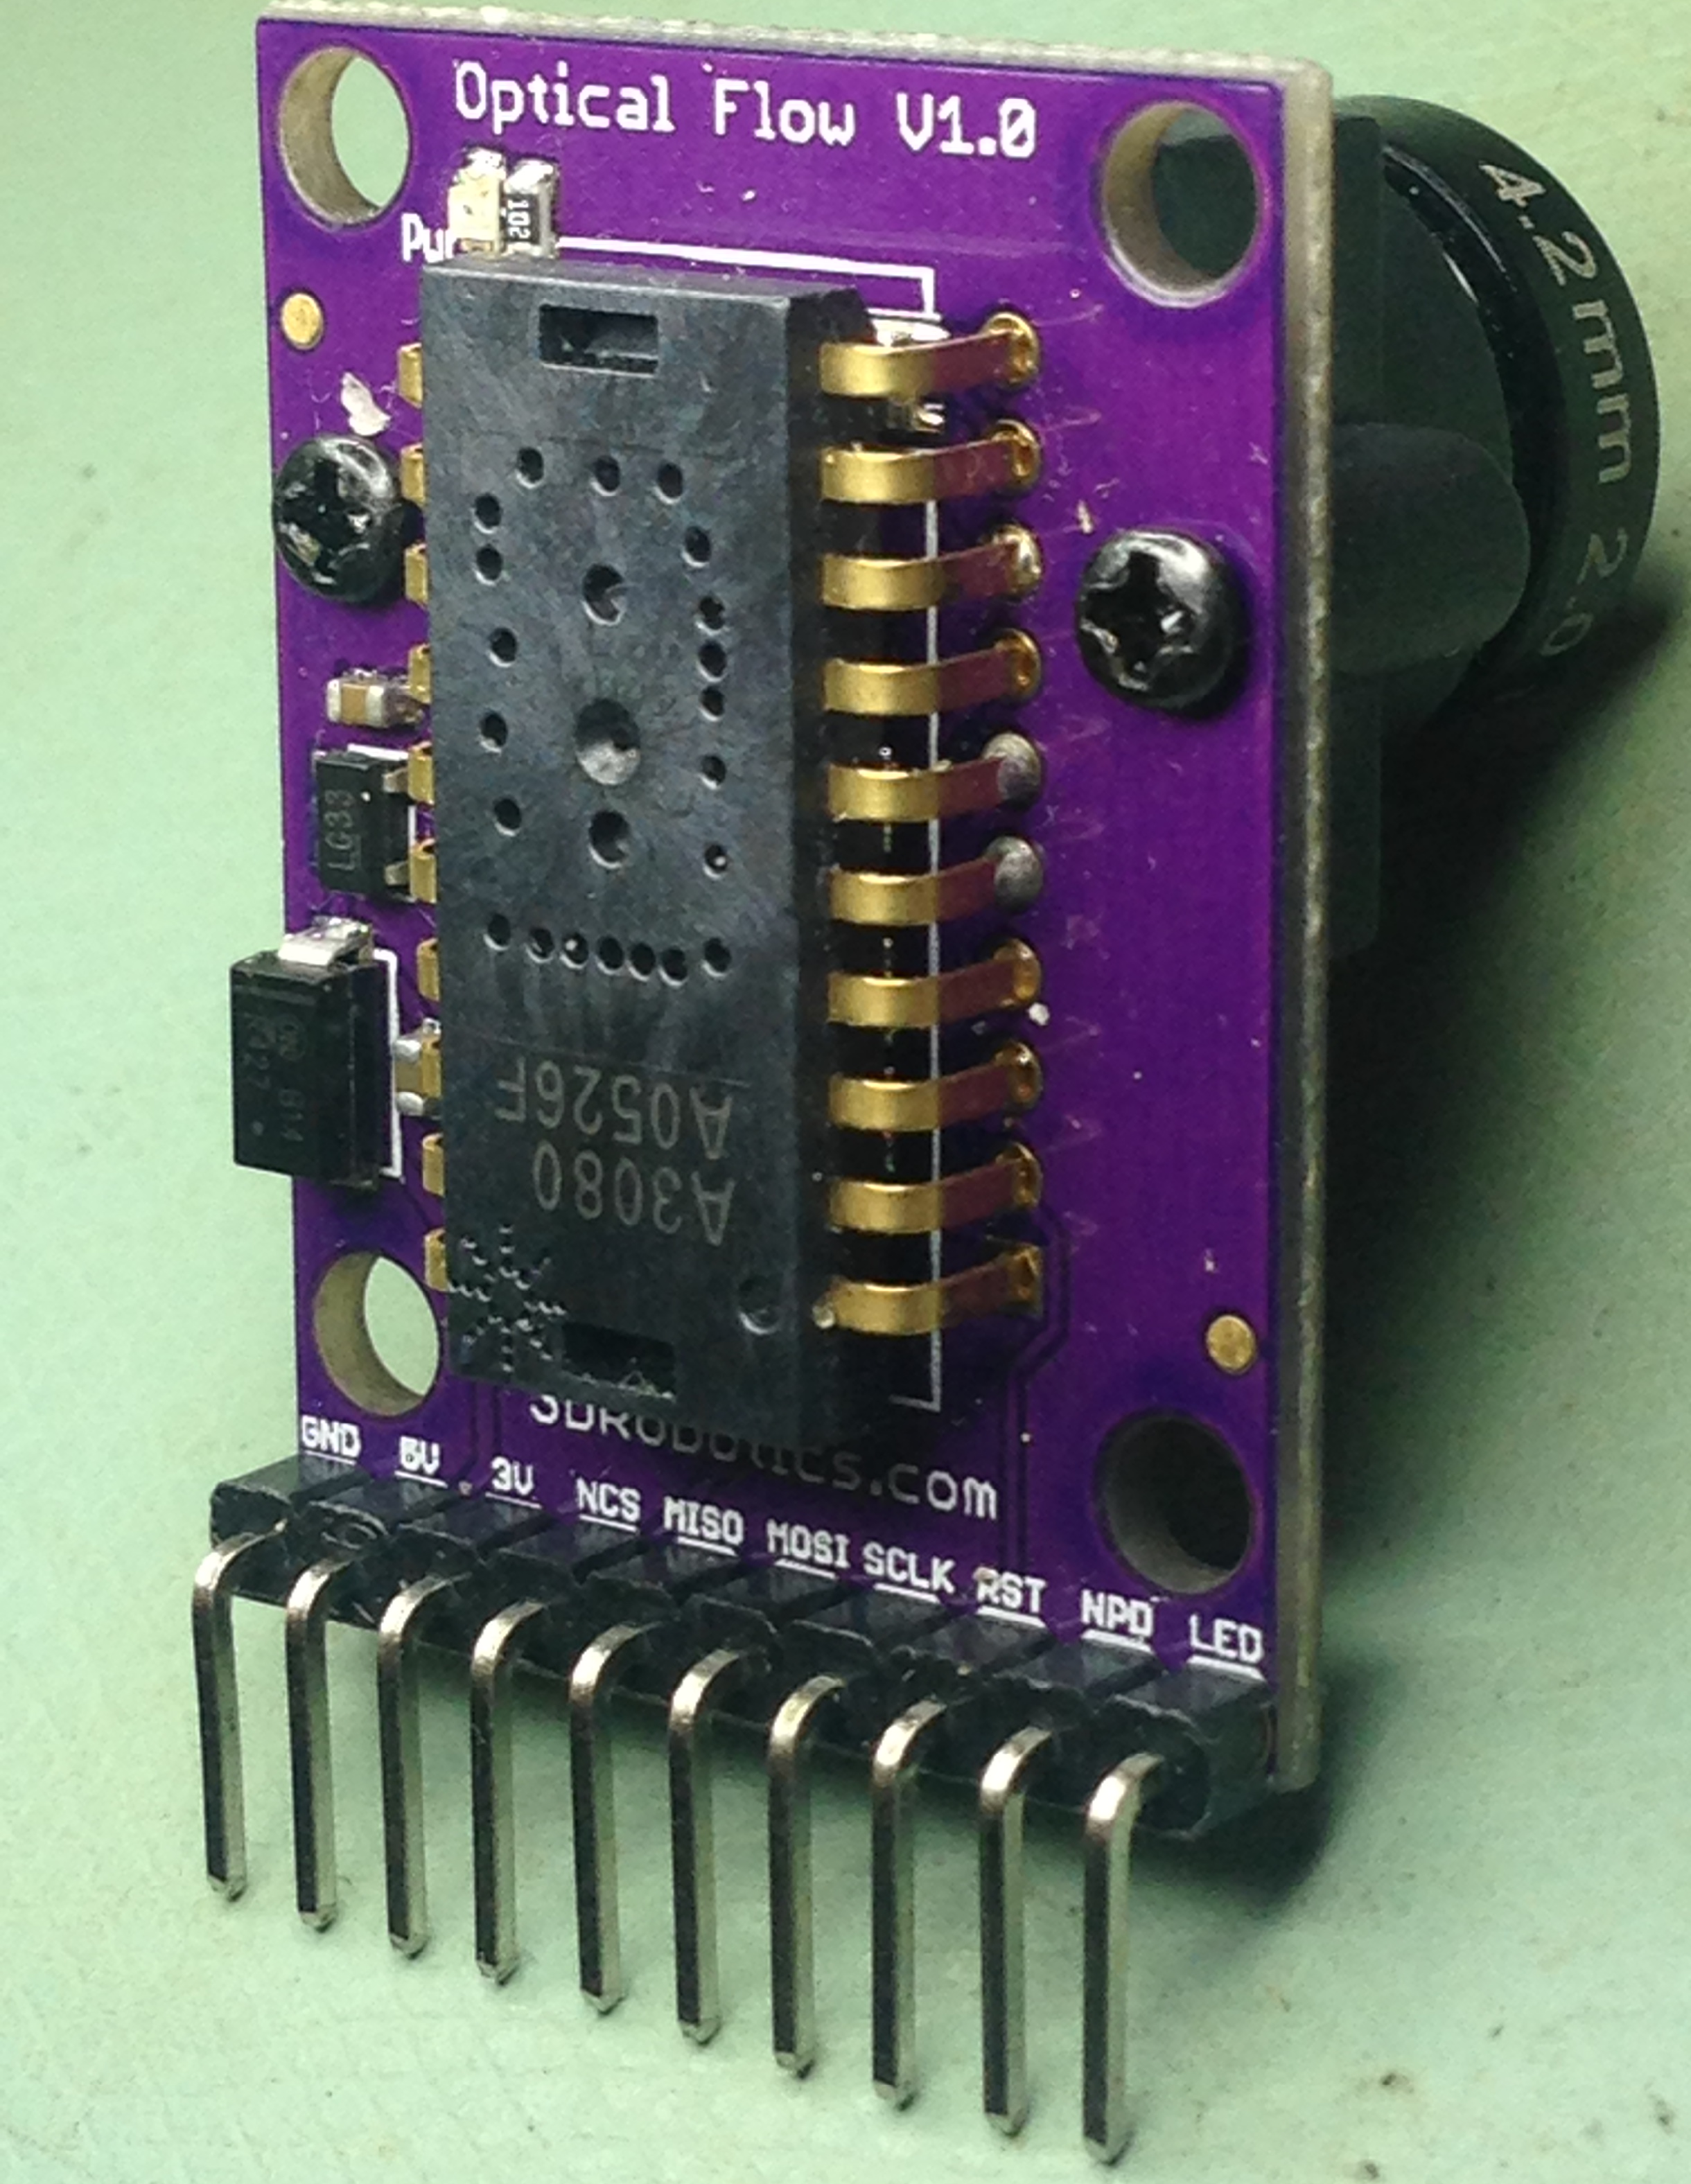
\includegraphics[width=0.4\textwidth]{OpticalFlowSensor}
\caption{Optical Mouse Sensor}
\label{OpticalFlowSensor}
\end{figure}%
%
%\subsubsection{Accumulated \(Z^W\)-axis data calibration}
%
Sensor ANDS-3080 has a programmable frame rate of over 6400 fps. With a lens mounted, this optical flow sensor can theoretically adjust its working distance from zero to one meter. Both of the raw 30-by-30 image frame and the calculated motion results could be retrieved from the optical flow sensor in two different working modes. In the \enquote{image burst} mode, the raw 30-by-30 image frames form a 10 fps live video, helping adjust the lens for a better focus. Whereas in the \enquote{motion burst} mode, the calculated motion results offers accumulation data for both of the sensor's \(x\)-axis and \(y\)-axis.
\\\\%
Concretely as shown in figure \ref{MountedTrackingModuleObservingRail}, only the \(y\)-axis accumulated data is used as the accumulated \(Z^W\)-axis data in the world coordinate, whereas the \(x\)-axis accumulation is always zero (no motion on the \(x\)-axis. Employing the \enquote{motion burst} mode, on ever update, the world coordinate \(Z^W\) could be written as%
%
\begin{equation}
%
Z^W = Z^W_0 + ratio*y^{acc} = Z^W_0 + ratio*(y_{\text{\_all\_previous}} + y_{\text{\_new\_updated}})
%
\end{equation}
%
where \(Z^W_0\) denotes the beginning point of accumulating (concretely at the closest end of the rail to dots pattern), \(ratio\) maps the \enquote{unit one} from \(y\)-axis to the \(Z^W\)-axis, \(y^{acc}\) denotes the accumulated \(y\)-axis movement by data retrieved from the optical flow sensor, which equals to the sum of all previous values and the new updated value.
%
%\subsection{Bluetooth Low Energy for wireless communication}
%
ZigBee, Bluetooth, and Bluetooth Low Energy (BLE) are three most commonly used Personal Area Network (PAN) wireless standards to choose from when wireless communication is needed. ZigBee runs on a mesh topology network (star and point-to-point are the other two basic topologies), which means that the information travels on a web of multiple nodes. Whereas Bluetooth and BLE are famous as point-to-point networking standard, which suits better for this project, from Optical-Flow sensor to PC.
\\\\%
There are huge differences between BLE and \enquote{classic} Bluetooth; despite falling under the same name, they are entirely different technologies. Bluetooth consumes more power and transmits farther and with more data. It is suited for streaming media such as playing music on Bluetooth speakers or taking a call through a Bluetooth headset.
%
\begin{figure}[H]
\centering
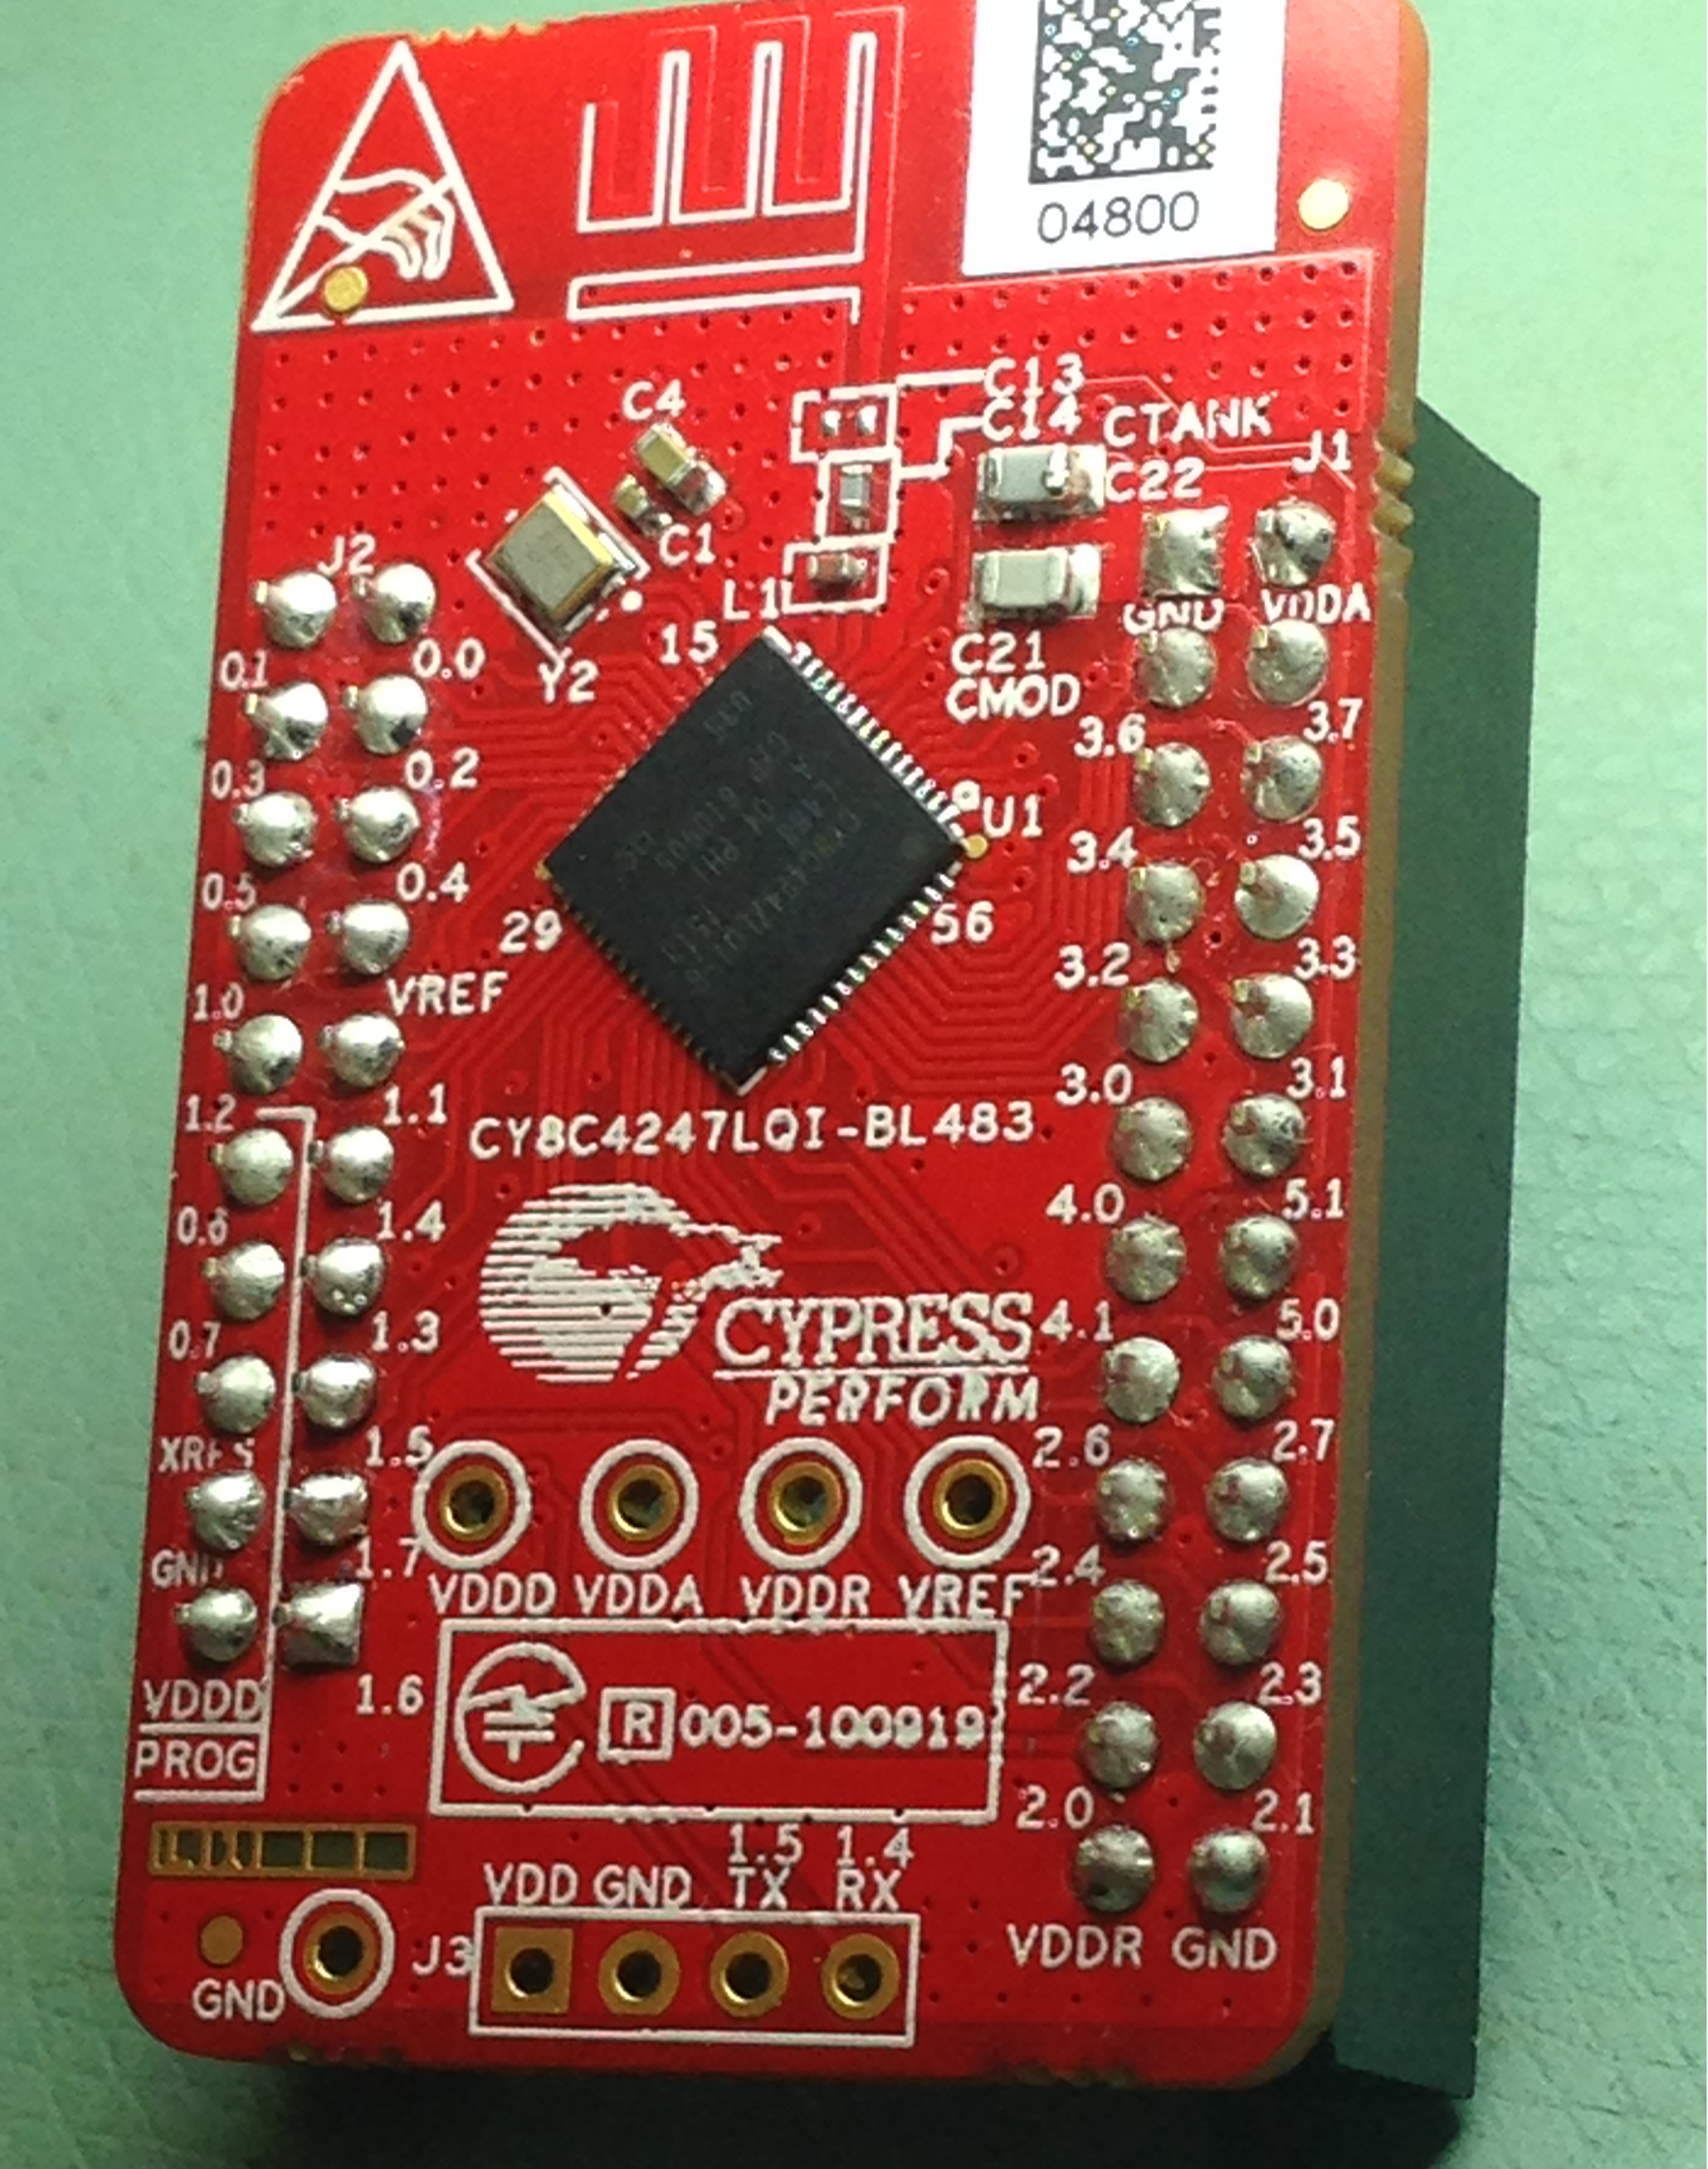
\includegraphics[width=0.4\textwidth]{PSoC_BLE_Module}
\caption{Cypress PSoC BLE Module}
\label{PSoC_BLE_Module}
\end{figure}%
%
Whereas BLE transmits less data over shorter distances using much less power than Bluetooth. Both of the transmission frequency and the amount of data to transfer per time are controllable by developer for BLE communication.
\\\\
%
As for the wireless data transmission in this project, with the \(x\)/\(y\) accumulation data being to transfer, the amount of data to transfer per time is only two bytes. Moreover, the maximum frame rate of optical flow sensor ANDS-3080 is 6400 fps, which means the transmission frequency cannot be faster than 6400 Hz (we do not need that fast in the meantime). In short, BLE is finally chosen as the wireless networking to transfer data from the optical flow sensor to PC. Concretely, the Cypress PSoC BLE Module is used, with a 10KB maximum throughput that is enough for the demand in this project, as shown in figure \ref{PSoC_BLE_Module}.
%
%\subsubsection{BLE Programming based on Protocol}
%
BLE is a low-power, short-range, low-data-rate wireless communication protocol. Unlike Bluetooth application that only the high level connection needs to be concerned, the BLE application developing needs low level programming, more complex but offering more control space for developer. Figure \ref{BLE_Protocol_Stack} shows the BLE Protocol Stack that BLE developers need to refer to.
%
\begin{figure}[H]
\centering
\includegraphics[width=0.7\textwidth]{BLE_Protocol_Stack}
\caption{BLE Protocol Stack \cite{Cypress15}}
\label{BLE_Protocol_Stack}
\end{figure}%
%
Cypress BLE Module helps handle the lowest hardware controller section (PHY, LL, HCI) and part of the firmware host section (L2CAP, ATT, SM), so that developers only need to take care of the GAP and GATT layers. GAP provides an application-oriented interface that determines whether the device acts as a BLE link \enquote{Central} or \enquote{Peripheral}, and configures the underlying layers accordingly. Whereas GATT defines methods to access data defined by ATT layer ( \enquote{Client} to receive or \enquote{Sever} to send).
\\\\%
Concretely for the BLE programming in this project, on the GPA layer, the BLE module continuously retrieving data from Optical-Flow sensor is the \enquote{Peripheral} that advertises to a Central, while a BLE dongle (receiver connected on PC) is the \enquote{Central} that scans for advertisements from GAP Peripherals and is going to establish the connection with the BLE module. Whereas on the GATT layer, the BLE module is the \enquote{Sever} that contains data and the dongle on PC works as a \enquote{Client} to receive data.
\\\\%
To program on the PC side, both of the command sending and data receiving are through the serial port which connects the BLE dongle. Both of the output command to send and received the input data are packaged in a center format, which means for every command about BLE control, there must be a method to package it and a corresponding decoding method to extract valid data. All of the commands that need to be managed are to handle GATT data transmission and GAP connection problem. After GATT and GAP setting, concretely, the optical flow sensor works at a sampling rate of 2000Hz and the BLE communication speed is 100 updates per second, i.e., \(Z^W\) is updated at 100Hz.
%
%
\subsection{PCB Joint, Power Supply and Illumination}
%
Figure \ref{SenSinglePCB} shows the PCB combining and powering (3.3 \texttildelow \, 16V flexible voltage input) for a PSoC BLE module, an OF sensor, and a LED for OF sensor illumination. Figure \ref{BLE_OF_TrackingModule_Overview} shows the overview of the BLE Optical-Flow Tracking Module.
%
\begin{figure}[H]
\centering
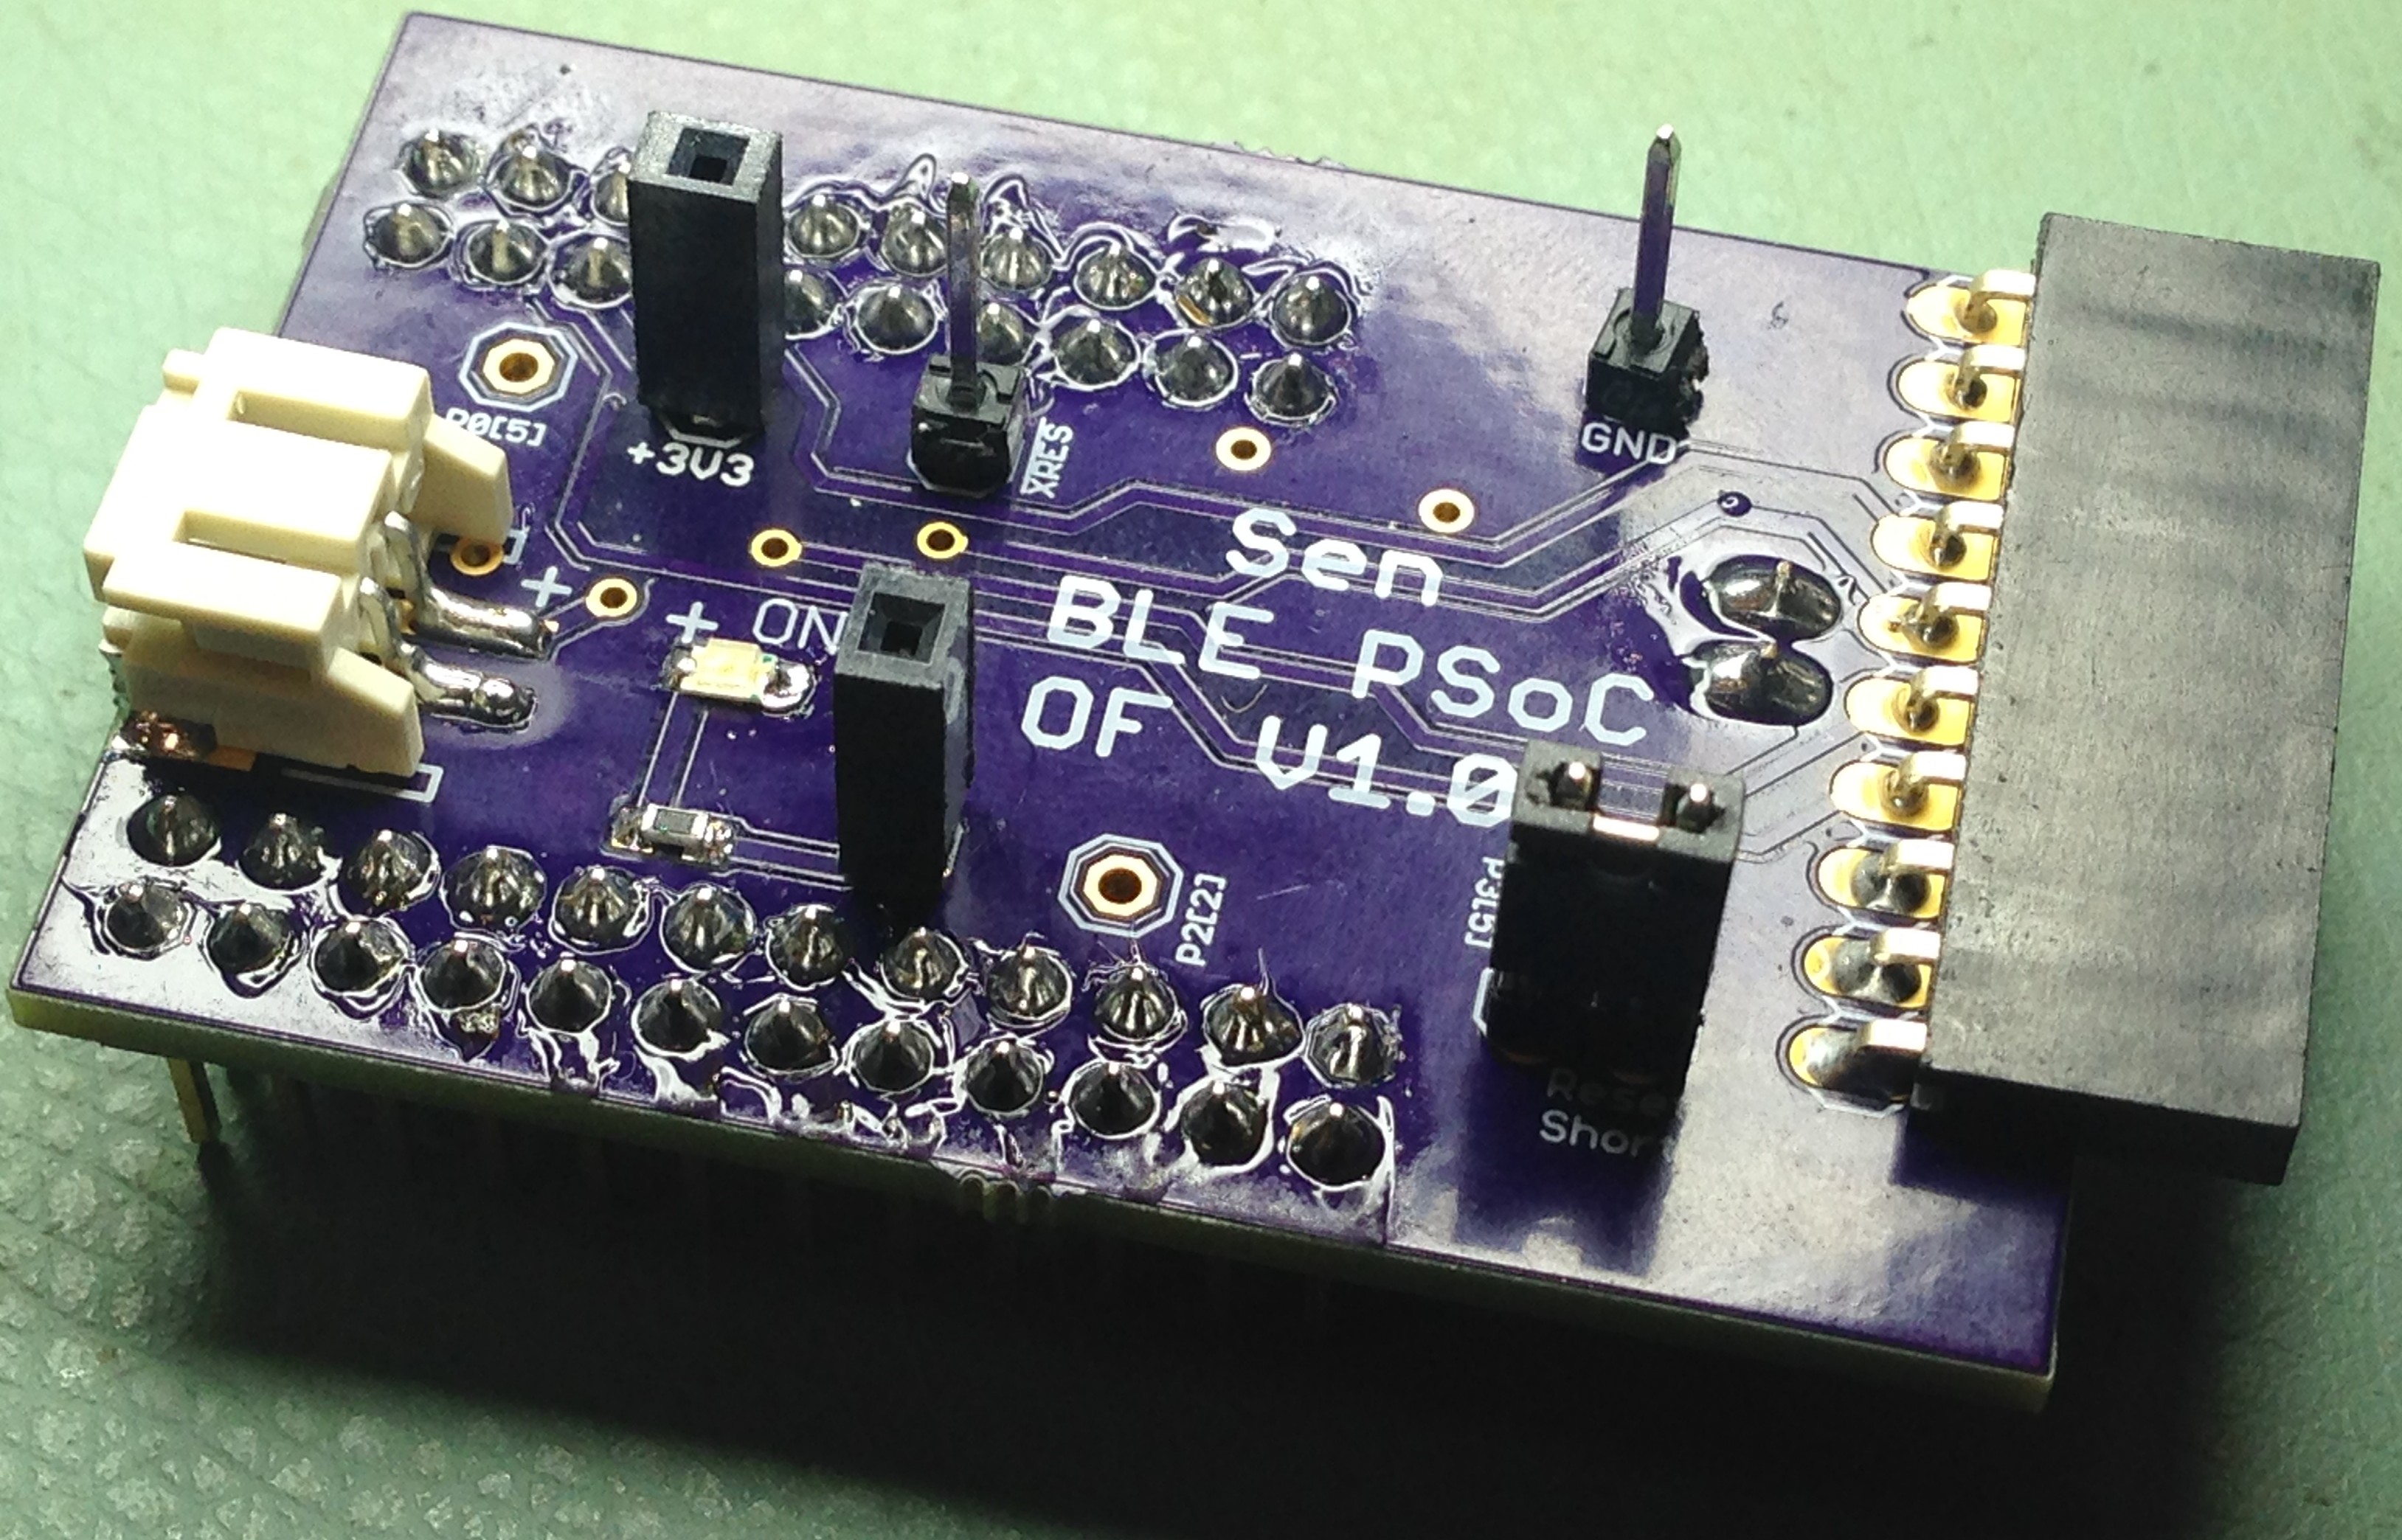
\includegraphics[width=0.7\textwidth]{SenSinglePCB}
\caption{PCB: joint \& power supply}
\label{SenSinglePCB}
\end{figure}%
%
%
 \begin{figure}[H]
\hspace*{-0.3cm}
\centering
\subfloat[Front Side][Front]{
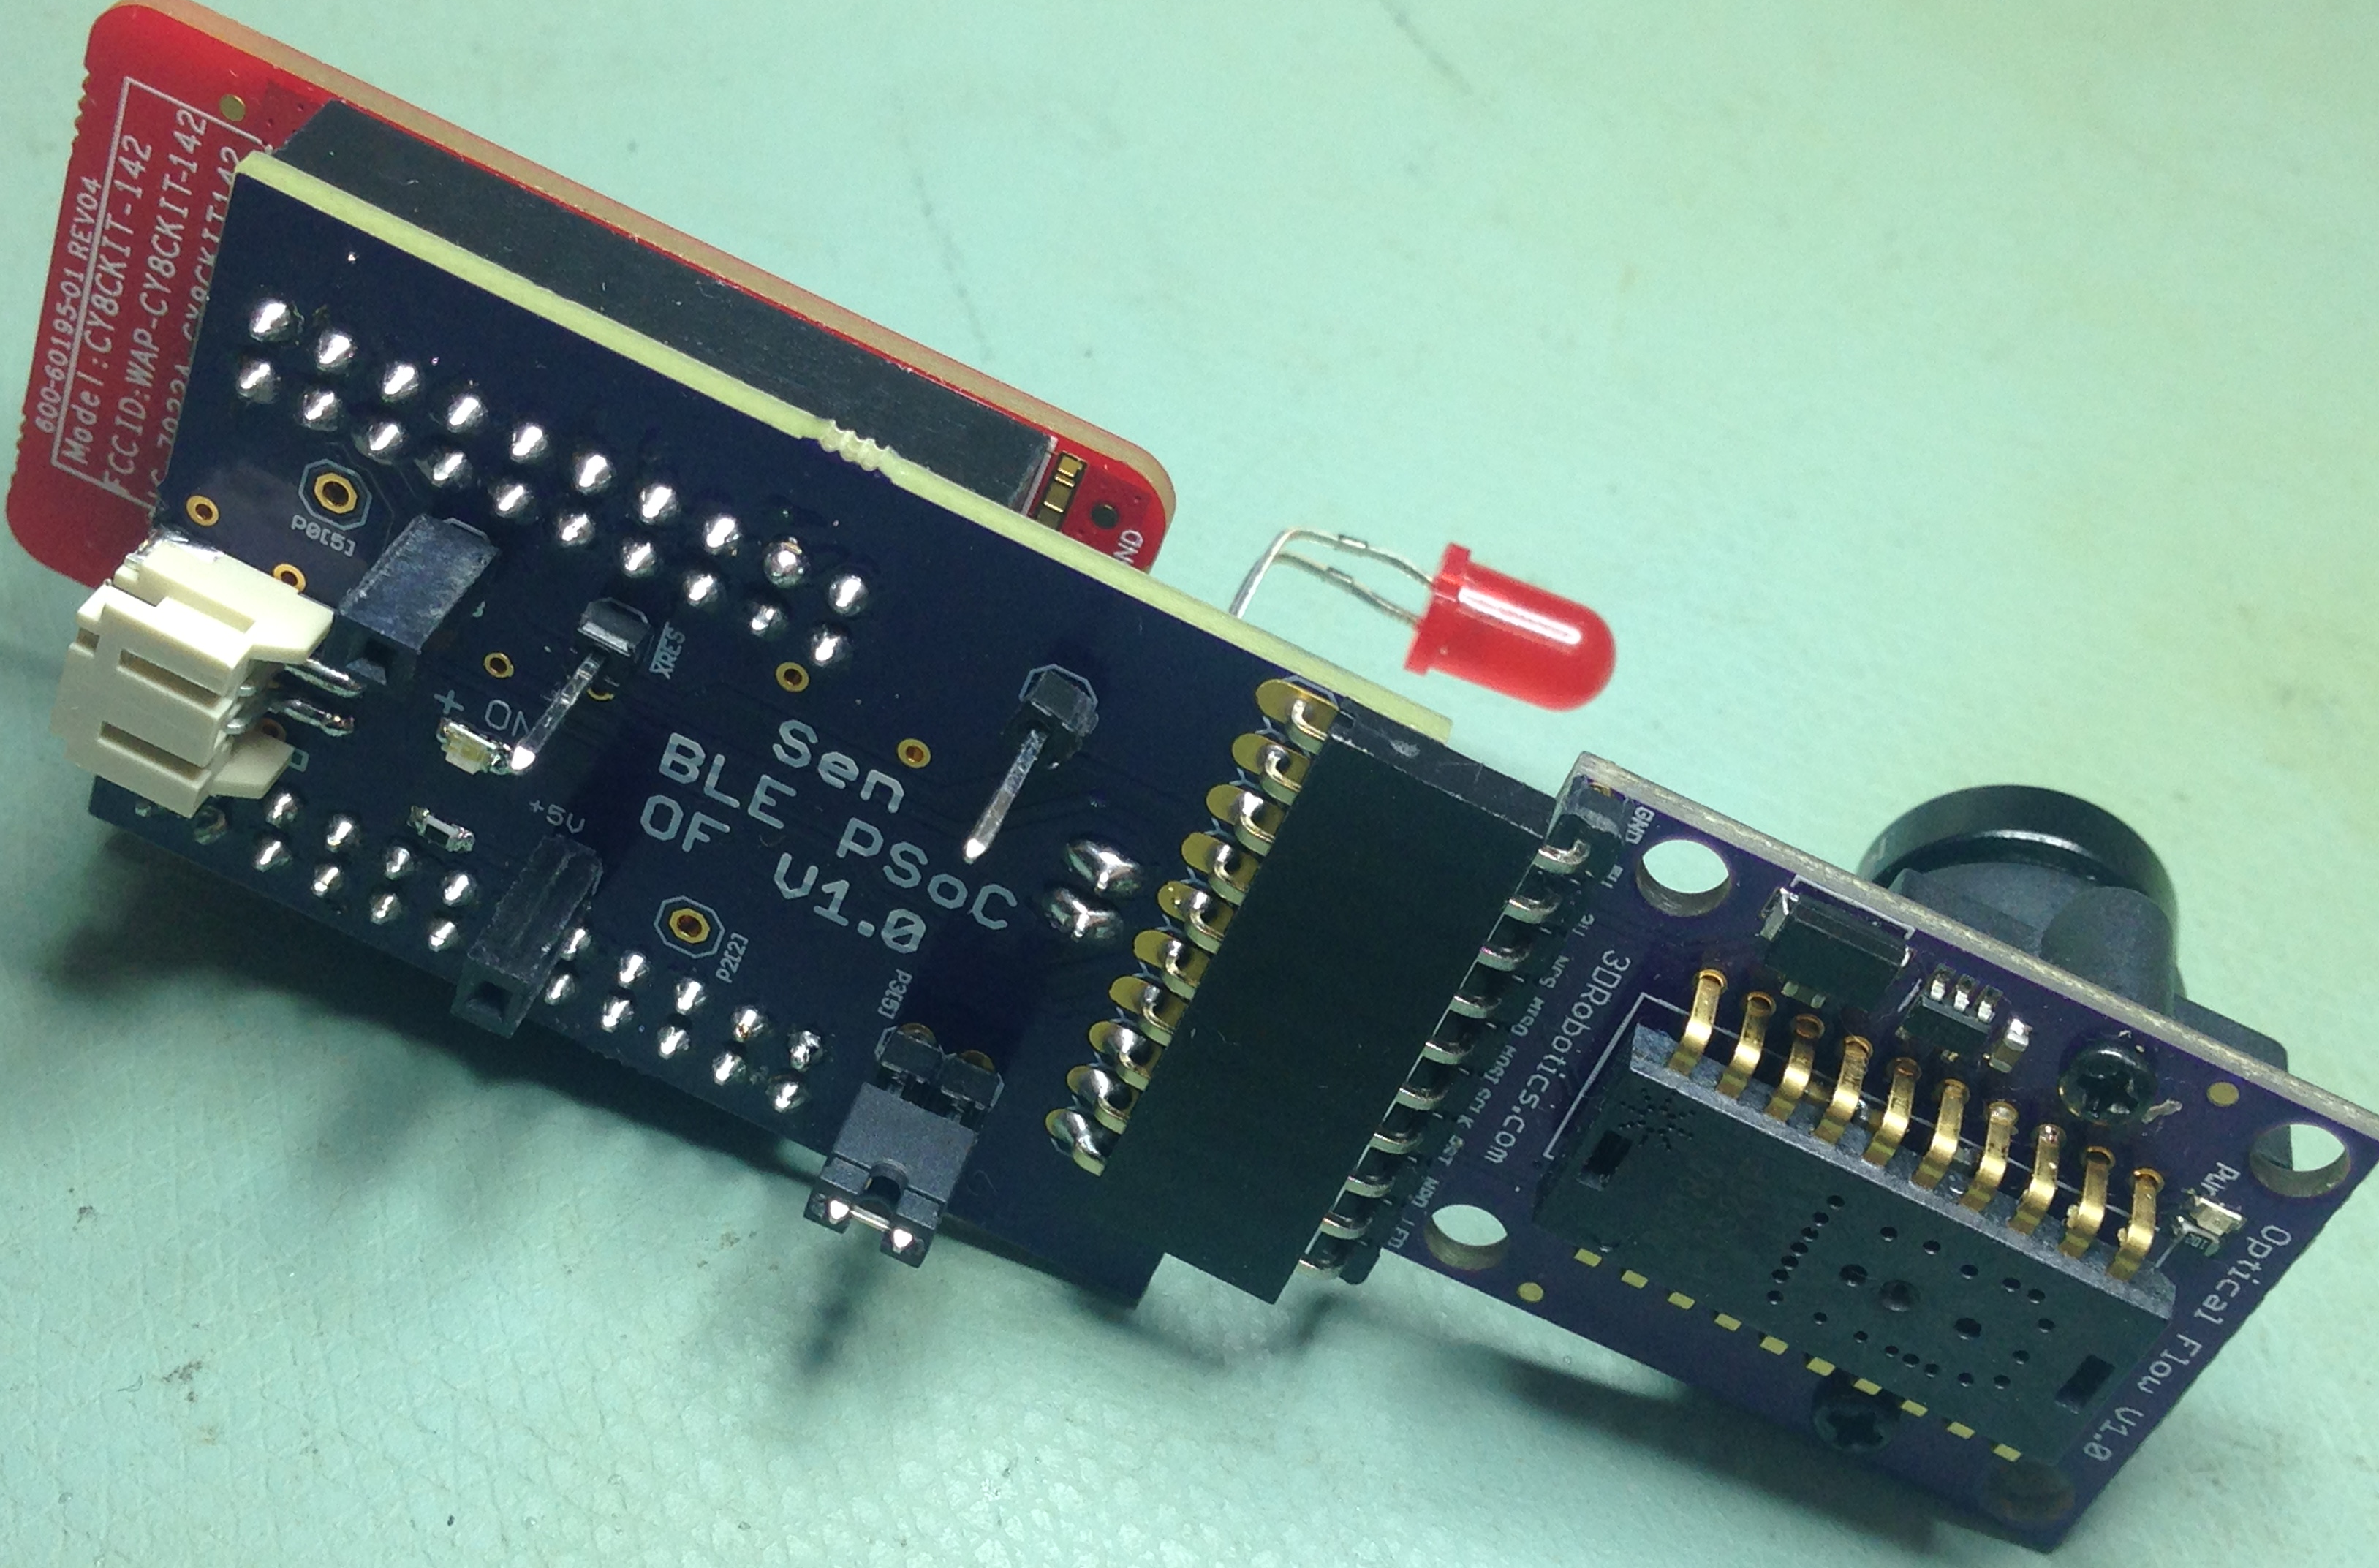
\includegraphics[width=0.54\textwidth, height = 0.35\textwidth]{combinedModuleFace}
\label{combinedModuleFace}}
%\qquad
\subfloat[Back Side][Back]{
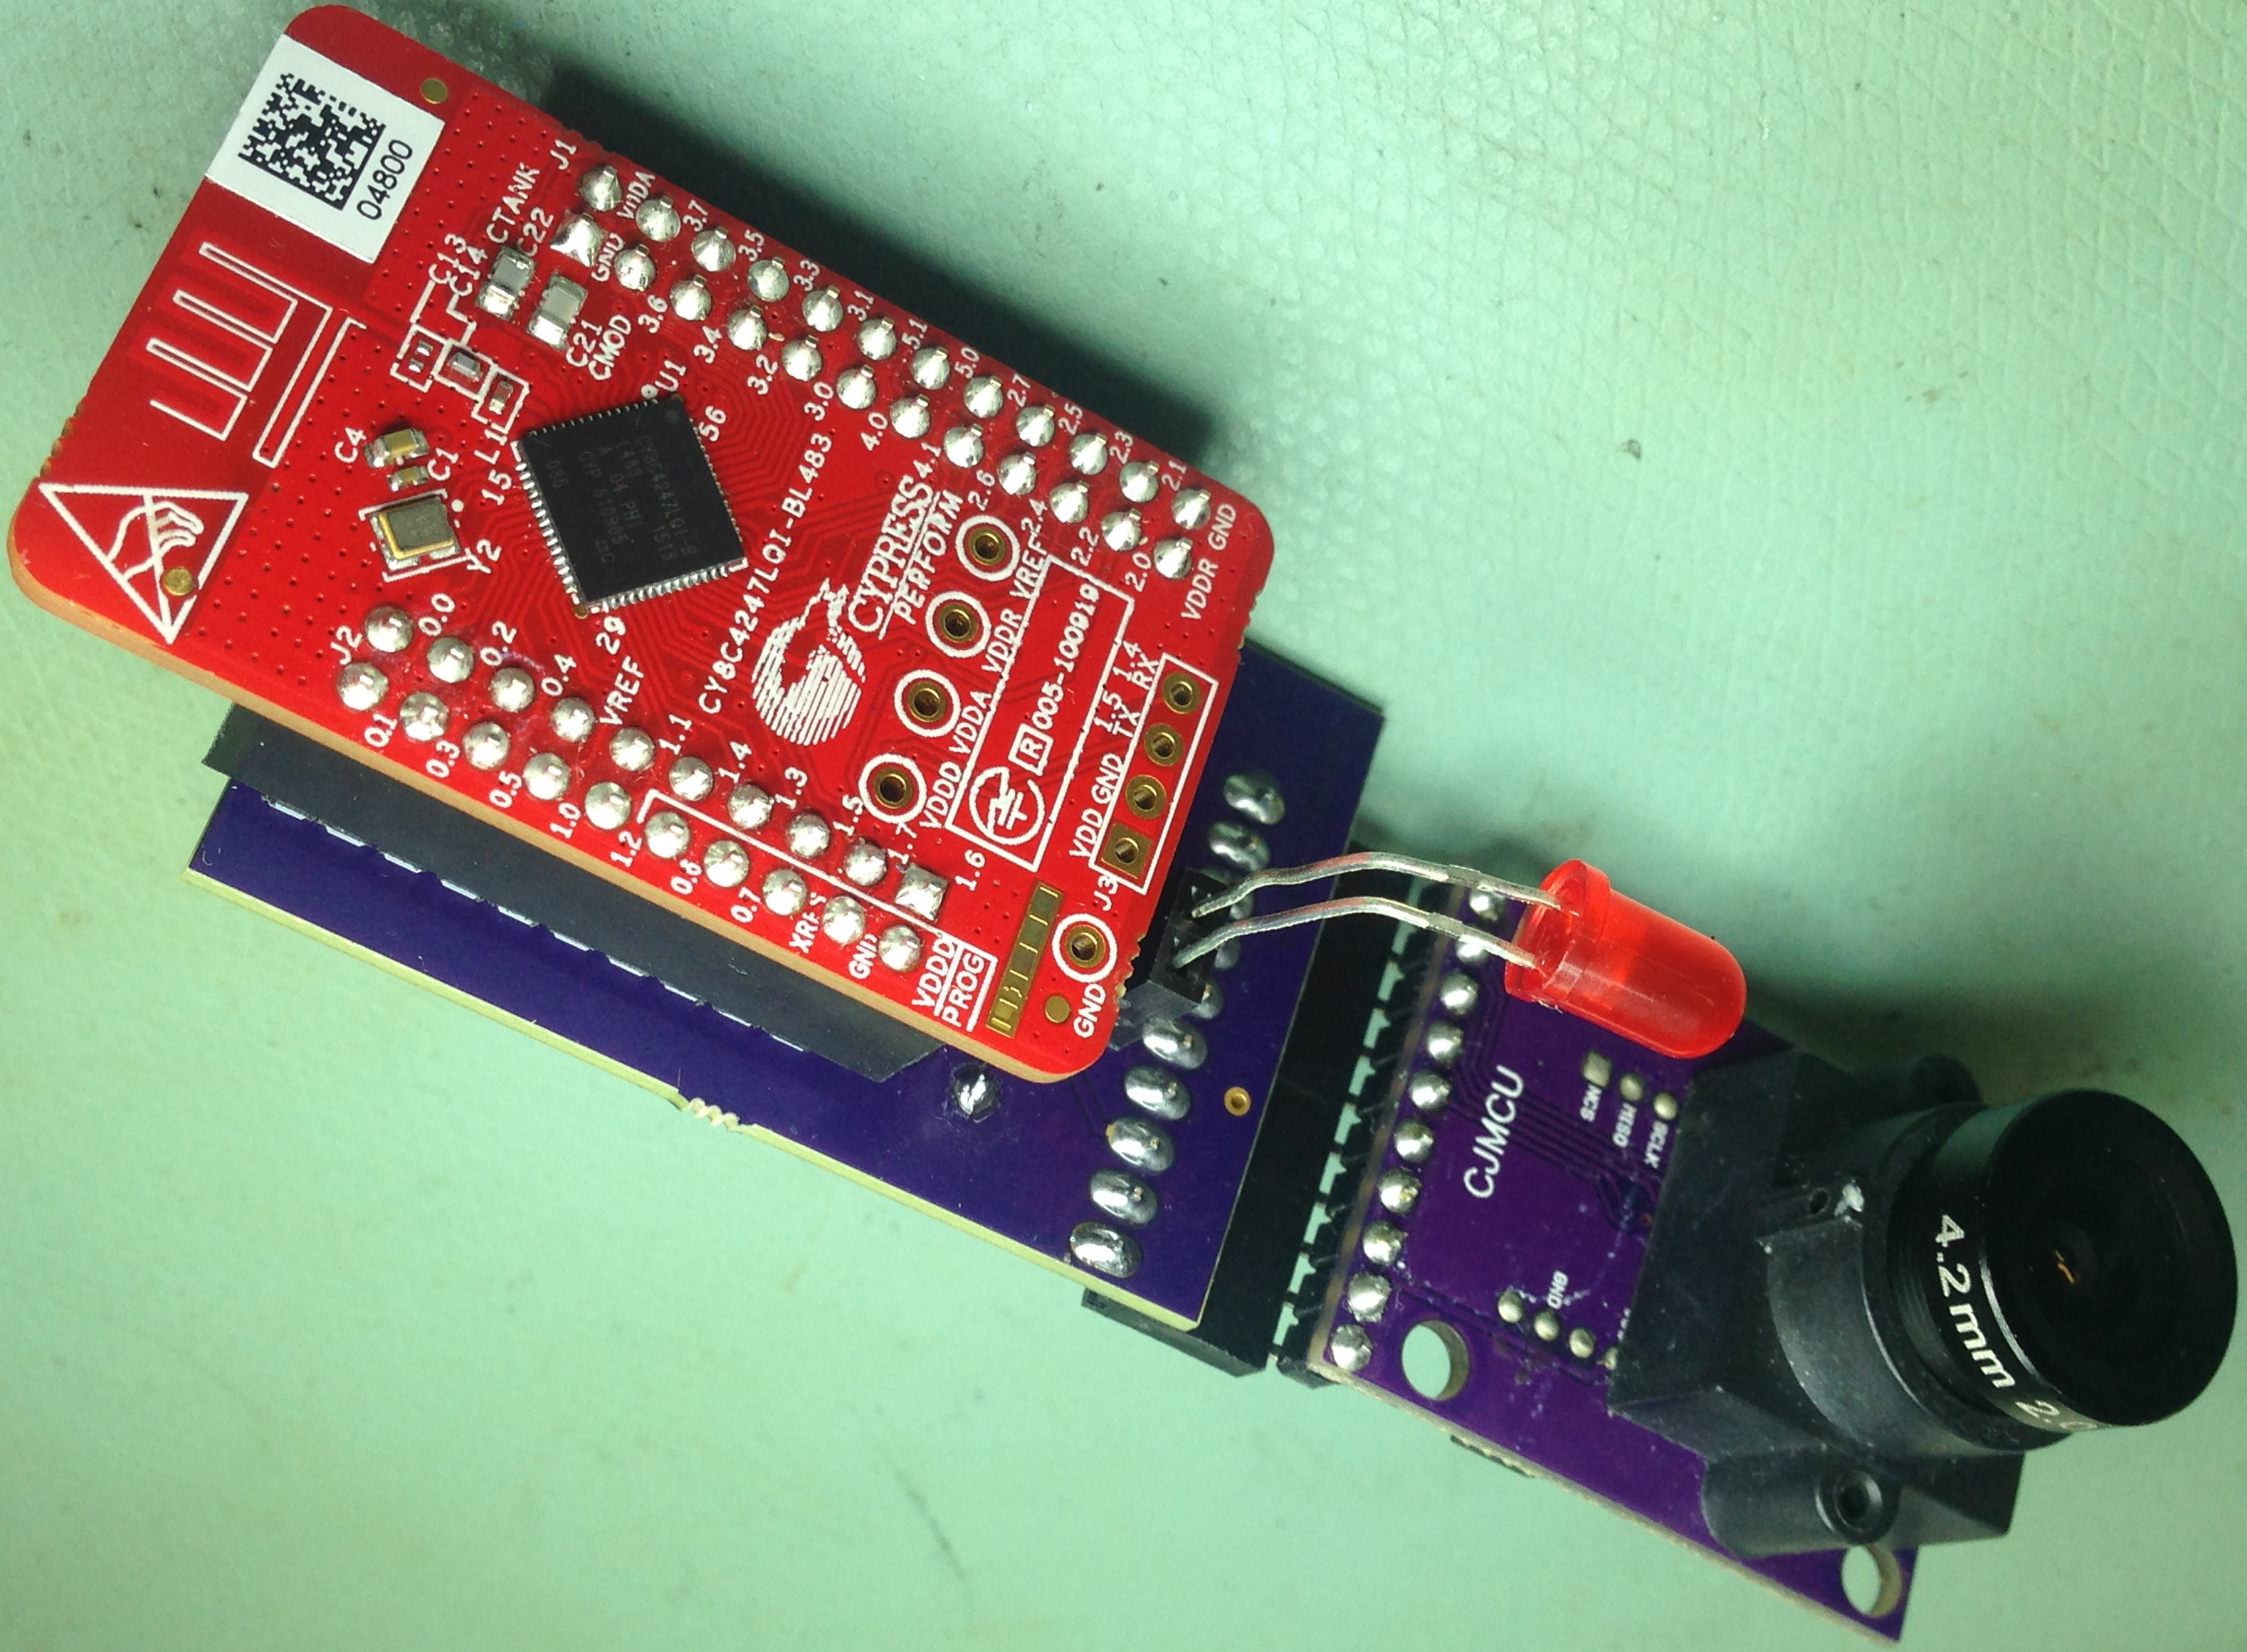
\includegraphics[width = 0.47\textwidth, height = 0.35\textwidth]{combinedModuleBack}
\label{combinedModuleBack}}
%
\caption{Overview of BLE OF Tracking Module}
\label{BLE_OF_TrackingModule_Overview}
\end{figure}%
%
%
%
%
%
%
%
%Chapter 4: results for 3 types of RGB-D cameras.\\
%Chapter 5: conclusion\\





































 
%\copyrightnotice
%% Chapter 3
\chapter{Conclusion and Future Work} % Main chapter title
\label{sens_ConclusionAndFutureWork} 

\section{Conclusion}
The depth sensor technologies opens a new epoch for 3D markets. Ever since the Microsoft brought the low-cost depth camera Kinect into consumer market, RGB-D cameras are famous in in research areas of HCI, and an accurate RGB-D camera calibration is now important in computer vision. However, the traditional camera calibration methods are not ideal on accuracy and efficiency. They do not cover all pixels of a sensor, and did not consider the problem of \enquote{Depth Distortion} either. Besides, those methods need the distortion removal to be a second step after raw 3D reconstruction (from a pinhole camera matrix), which is not an efficient way displaying the 3D reconstruction in real-time.
\\\indent
In this thesis, a novel per-pixel calibration method with look-up table based 3D reconstruction in real-time is introduced, using a rail calibration system. Instead of using the traditional pinhole camera model, two polynomial mapping models are employed in this calibration method. The first model is the two-dimensional \(4^{th}\) order polynomial mapping from \(R/C\) to \(X^W/Y^W\) during the frames data collection, which takes care of the removal of lens distortions; and the second model is the linear mapping from \(D\) to \(Z^W\), which can handle \enquote{depth distortion}. The method consists of two big steps: \(X^WY^WZ^W+D\) data collection and mapping parameters determination. \(D\) is simply from depth streams. \(Z^W\) is from external based on the camera's position on the rail. And the undistorted (\(X^W, \, Y^W\)) are from the transformation of \(R/C\) by a \(4^{th}\) order polynomial mapping model, during which lens-distortions could be removed. This method is claimed as \enquote{data-based} calibration method, because both of the two mapping models are determined and calculated by real streams data from the camera. 
\\\indent
With the fewest calculations, the undistorted 3D world coordinates (\(X^\text{W}, \, Y^\text{W}, \, Z^\text{W}\)) for every single pixel could be looked up in real-time based on \(D\) from a \(column\)-by-\(row\)-by-\(6\) look-up table. Two out of six parameters \(a/b\) are to determine the per-pixel \(Z^W\), which is generated from per-pixel depth value \(D\); and the other four parameters \(c/d/d/f\) are to determine the per-pixel \(X^W/Y^W\) respectively, which are mapped by per-pixel linear beam equation from the per-pixel \(Z^W\). Note that \enquote{real-time} here means being able to show an undistorted frame in 3D world space before the start of the second frame processing. The data-based per-pixel calibration method could be applied universally on any RGB-D cameras. With the alignment of RGB pixels using a pinhole camera matrix, it could even work on the combined 3D camera of a random Depth sensor and a random RGB sensor.
%%%%%%%%%%%%%%%%%%%%%%%%%%%%%%%%%%%%%%%%%%%%%%%%%%
%%%%%%%%%%%                                                                %%%%%%%%%%%%%%%%%
%%%%%%%%%%     5.2  Future Work                                    %%%%%%%%%%%%%%%%%%%%
%%%%%%%%%%%                                                                %%%%%%%%%%%%%%%%%%
%%%%%%%%%%%%%%%%%%%%%%%%%%%%%%%%%%%%%%%%%%%%%%%%%%%
\section{Future Work}
%
The rail calibration system and per-pixel calibration method with LUT-based real-time 3D reconstruction could be applied universally to all kinds of RGB-D cameras. With a more precise calibration system and corresponding DIP technologies, there could be a huge improvement space for calibration accuracy. Hardware improvement is sometimes more important than a software updating. Concretely the system in the lab now can only handle a working distance \(Z^W\) from 1.165m to 2.565m. Considering that the depth resolution deteriorates notably with depth, it might not be linear relationship between \(D\) and \(Z^W\) for every single pixel, when the depth \(D\) value goes much further than the limit of the rail. In that case, the per-pixel \(D\) to \(Z^W\) mapping could be changed from singular linear to segmented mapping function that has non-linear section when \(D\) gets larger than a certain value.
\\\indent
Not only the rail, the planar pattern could also be changed based on the resolution of the camera (\textit{e.g.}, size of the dots and side distance of the unit square-shaped of the uniform grid could be larger when calibrating camera with a supper high resolution). A two dimensional object is totally enough for calibrating KinectV2, because the NearIR stream have same pixels' distortions with the depth stream. However, if NearIR stream could not be used to extract points \(R/C\) in image space (\textit{e.g.} a structured light based depth sensor) and the size (pixel numbers) of the RGB sensor does not share the same one with the depth sensor, we could make the planar pattern into a \enquote{three dimension mode}: change the printed dots into real whole such that the depth stream could detect a difference between the \enquote{dots} and \enquote{white background}. Instead of using a laser distance measurer to manually input \(Z^W\) into every frame during the frame data collection, we could add a tracking module onto the rail to active the frame collection by software. In this way, not only \(Z^W\) could be traced by the tracking module, but also the frame collection could be automatically done by the activation of the tracking module, to record one frame data after moving every certain distance. 
\\\indent
Besides the hardware enhancement, softwares like DIP process can also be improved. The order of polynomial model that help map from image space \(R/C\) to world space \(X^W/Y^W\) could also be heightened for a better accuracy, as long as there will be enough calibrating points to offer the coordinates pairs of both image space and world space. Considering the possible lens-distortions of the RGB sensor, the high order polynomial mapping could also be applied into the alignment from RGB sensor pixels to depth sensor pixels, after the first step of pinhole camera model mapping.

































%\copyrightnotice



\backmatter

\onehalfspacing
%\begin{singlespace} % Bibliography must be single spaced
\bibliographystyle{plain}    % Set the bibliography style. agu04, plain, alpha, etc.
\bibliography{SenResource}
%\end{singlespace}

%\chapter{Vita}
%A brief vita goes here.












\end{document}










